%%
%% This is file `sample-sigconf.tex',
%% generated with the docstrip utility.
%%
%% The original source files were:
%%
%% samples.dtx  (with options: `sigconf')
%% 
%% IMPORTANT NOTICE:
%% 
%% For the copyright see the source file.
%% 
%% Any modified versions of this file must be renamed
%% with new filenames distinct from sample-sigconf.tex.
%% 
%% For distribution of the original source see the terms
%% for copying and modification in the file samples.dtx.
%% 
%% This generated file may be distributed as long as the
%% original source files, as listed above, are part of the
%% same distribution. (The sources need not necessarily be
%% in the same archive or directory.)
%%
%% The first command in your LaTeX source must be the \documentclass command.
\documentclass[sigconf]{acmart}
\usepackage[tight,footnotesize]{subfigure}
\usepackage{makecell}
\usepackage{xspace}
%%
%% \BibTeX command to typeset BibTeX logo in the docs
\AtBeginDocument{%
  \providecommand\BibTeX{{%
    \normalfont B\kern-0.5em{\scshape i\kern-0.25em b}\kern-0.8em\TeX}}}

%% Rights management information.  This information is sent to you
%% when you complete the rights form.  These commands have SAMPLE
%% values in them; it is your responsibility as an author to replace
%% the commands and values with those provided to you when you
%% complete the rights form.
\setcopyright{acmcopyright}
\copyrightyear{2018}
\acmYear{2018}
\acmDOI{10.1145/1122445.1122456}

%% These commands are for a PROCEEDINGS abstract or paper.
\acmConference[Woodstock '18]{Woodstock '18: ACM Symposium on Neural
  Gaze Detection}{June 03--05, 2018}{Woodstock, NY}
\acmBooktitle{Woodstock '18: ACM Symposium on Neural Gaze Detection,
  June 03--05, 2018, Woodstock, NY}
\acmPrice{15.00}
\acmISBN{978-1-4503-XXXX-X/18/06}


%%
%% Submission ID.
%% Use this when submitting an article to a sponsored event. You'll
%% receive a unique submission ID from the organizers
%% of the event, and this ID should be used as the parameter to this command.
%%\acmSubmissionID{123-A56-BU3}

%%
%% The majority of ACM publications use numbered citations and
%% references.  The command \citestyle{authoryear} switches to the
%% "author year" style.
%%
%% If you are preparing content for an event
%% sponsored by ACM SIGGRAPH, you must use the "author year" style of
%% citations and references.
%% Uncommenting
%% the next command will enable that style.
%%\citestyle{acmauthoryear}

%%
%% end of the preamble, start of the body of the document source.
\begin{document}

\newcommand\pname{\textbf{ProjectName}\xspace}
%%
%% The "title" command has an optional parameter,
%% allowing the author to define a "short title" to be used in page headers.
\title{Containerized Serverless Functions with Initialization-less Booting for Serverless Computing}

%%
%% The "author" command and its associated commands are used to define
%% the authors and their affiliations.
%% Of note is the shared affiliation of the first two authors, and the
%% "authornote" and "authornotemark" commands
%% used to denote shared contribution to the research.


\author{Bowen Yan}
\authornote{Both authors contributed equally to this research.}
\email{yanbowen18@otcaix.iscas.ac.cn}
\affiliation{%
  \institution{University of Chinese Academy of Sciences}
  \city{Beijing}
  \country{China}
}

% \author{Lars Th{\o}rv{\"a}ld}
% \affiliation{%
%   \institution{The Th{\o}rv{\"a}ld Group}
%   \streetaddress{1 Th{\o}rv{\"a}ld Circle}
%   \city{Hekla}
%   \country{Iceland}}
% \email{larst@affiliation.org}

% \author{Valerie B\'eranger}
% \affiliation{%
%   \institution{Inria Paris-Rocquencourt}
%   \city{Rocquencourt}
%   \country{France}
% }

% \author{Aparna Patel}
% \affiliation{%
%  \institution{Rajiv Gandhi University}
%  \streetaddress{Rono-Hills}
%  \city{Doimukh}
%  \state{Arunachal Pradesh}
%  \country{India}}

% \author{Huifen Chan}
% \affiliation{%
%   \institution{Tsinghua University}
%   \streetaddress{30 Shuangqing Rd}
%   \city{Haidian Qu}
%   \state{Beijing Shi}
%   \country{China}}

% \author{Charles Palmer}
% \affiliation{%
%   \institution{Palmer Research Laboratories}
%   \streetaddress{8600 Datapoint Drive}
%   \city{San Antonio}
%   \state{Texas}
%   \country{USA}
%   \postcode{78229}}
% \email{cpalmer@prl.com}

% \author{John Smith}
% \affiliation{%
%   \institution{The Th{\o}rv{\"a}ld Group}
%   \streetaddress{1 Th{\o}rv{\"a}ld Circle}
%   \city{Hekla}
%   \country{Iceland}}
% \email{jsmith@affiliation.org}

% \author{Julius P. Kumquat}
% \affiliation{%
%   \institution{The Kumquat Consortium}
%   \city{New York}
%   \country{USA}}
% \email{jpkumquat@consortium.net}

%%
%% By default, the full list of authors will be used in the page
%% headers. Often, this list is too long, and will overlap
%% other information printed in the page headers. This command allows
%% the author to define a more concise list
%% of authors' names for this purpose.
\renewcommand{\shortauthors}{Trovato and Tobin, et al.}

%%
%% The abstract is a short summary of the work to be presented in the
%% article.
\begin{abstract}
Serverless computing is a new cloud computing execution model which enables users to focus on writing function codes without configuring and managing the hardware and software environment. 
Serverless computing starts the isolation sandboxes for executing functions based on an event-driven model, 
which requires higher startup efficiency for the functions running on the serverless computing platform. 
However, the startup of containerized serverless functions can take hundreds of milliseconds to seconds due to the creation of the isolation environment and initialization of the software environment, which does not satisfy the performance standard of the serverless computing platforms.

This paper proposes a fast function startup design based on the container checkpoint/restore technique. 
By restoring a containerized function instance from the checkpoint of previously executed function process, the time-consuming processes in the function startup phase are skipped. 
Furthermore, two strategies are proposed to boost the restore process: 
i) The \textit{isolation environment pooling} strategy pre-initializes and caches the namespace resources required by functions to speed up the construction process of the sandbox. ii) The \textit{memory shared mapping} strategy uses on-demand loading to restore memory data and share memory pages among multiple functions, which improves the efficiency of memory data recovery and reduces the memory footprint of functions. The evaluation shows that this paper can reduce the startup latency of the functions by up to 70\% compared to the default serverless function startup method. Furthermore, this system can significantly reduce the concurrent deployment latency and resource usage of serverless functions in the scenario of large-scale deployment of serverless functions. 
\end{abstract}

%%
%% The code below is generated by the tool at http://dl.acm.org/ccs.cfm.
%% Please copy and paste the code instead of the example below.
%%
\begin{CCSXML}
<ccs2012>
 <concept>
  <concept_id>10010520.10010553.10010562</concept_id>
  <concept_desc>Computer systems organization~Embedded systems</concept_desc>
  <concept_significance>500</concept_significance>
 </concept>
 <concept>
  <concept_id>10010520.10010575.10010755</concept_id>
  <concept_desc>Computer systems organization~Redundancy</concept_desc>
  <concept_significance>300</concept_significance>
 </concept>
 <concept>
  <concept_id>10010520.10010553.10010554</concept_id>
  <concept_desc>Computer systems organization~Robotics</concept_desc>
  <concept_significance>100</concept_significance>
 </concept>
 <concept>
  <concept_id>10003033.10003083.10003095</concept_id>
  <concept_desc>Networks~Network reliability</concept_desc>
  <concept_significance>100</concept_significance>
 </concept>
</ccs2012>
\end{CCSXML}

\ccsdesc[500]{Computer systems organization~Embedded systems}
\ccsdesc[300]{Computer systems organization~Redundancy}
\ccsdesc{Computer systems organization~Robotics}
\ccsdesc[100]{Networks~Network reliability}

%%
%% Keywords. The author(s) should pick words that accurately describe
%% the work being presented. Separate the keywords with commas.
\keywords{serverless computing; startup latency; checkpoint and restore;}

%% A "teaser" image appears between the author and affiliation
%% information and the body of the document, and typically spans the
%% page.

%%
%% This command processes the author and affiliation and title
%% information and builds the first part of the formatted document.
\maketitle
\section{introduction}

Serverless computing is another popular trend in the current cloud computing field.
Unlike the traditional IaaS\cite{iaas} or PaaS\cite{paas},
which relies on cloud users to manage virtual machines or configure the capacity and automatic scaling of applications.
Serverless computing delegates all the work of managing virtual machines, execution environments, and software environments to the cloud provider.
Cloud providers makes all the infrastructure management operations transparent to cloud users,
and users only need to focus on writing related functions, which frees users from the trouble of managing servers.
At the same time, serverless computing provides users with a more fine-grained billing model,
which charges based on the actual amount of resources consumed when providing services. Currently serverless computing has been supported by many platforms, including Amazon Lambda\cite{amazon}, IBM Cloud Func\-tion\cite{ibm},
Microsoft Azure Func\-tions\cite{microsoft} and Google Cloud Func\-tions\cite{google}.
At the same time, serverless computing has also developed rapidly in the open source community.
Serverless computing platforms represented by open source projects such as Open\-FaaS\cite{openfaas}, Kube\-less\cite{kubeless}, and K\-native\cite{knative} have received a lot of attention.

Since serverless computing uses an event-driven approach to handle requests,
that is, when each request comes,
a new serverless function is started to process it,
which places high requirements on the efficiency of serverless functions.
The current containerized serverless functions failed to achieve the low startup
latency due to the creation of the isolation environment and the initialization
of the software environment.
The figure\ref{default-proportion} shows the "Execution and Startup/Overall" ratio of five typical serverless
computing applications which are tested on the OpenFaas platform, thoes applications run on different language runtimes.
The experiment shows that on average, the execution latency only accounted for 31\% of overall latency,
at the same time, the overall latency of containerized serverless functions is usually over 100 milliseconds(as shown in the table\ref{overall-latency}),
which obviously cannot meet the high-performance requirements of serverless computing platforms.
\begin{figure}[t]
    \centering
    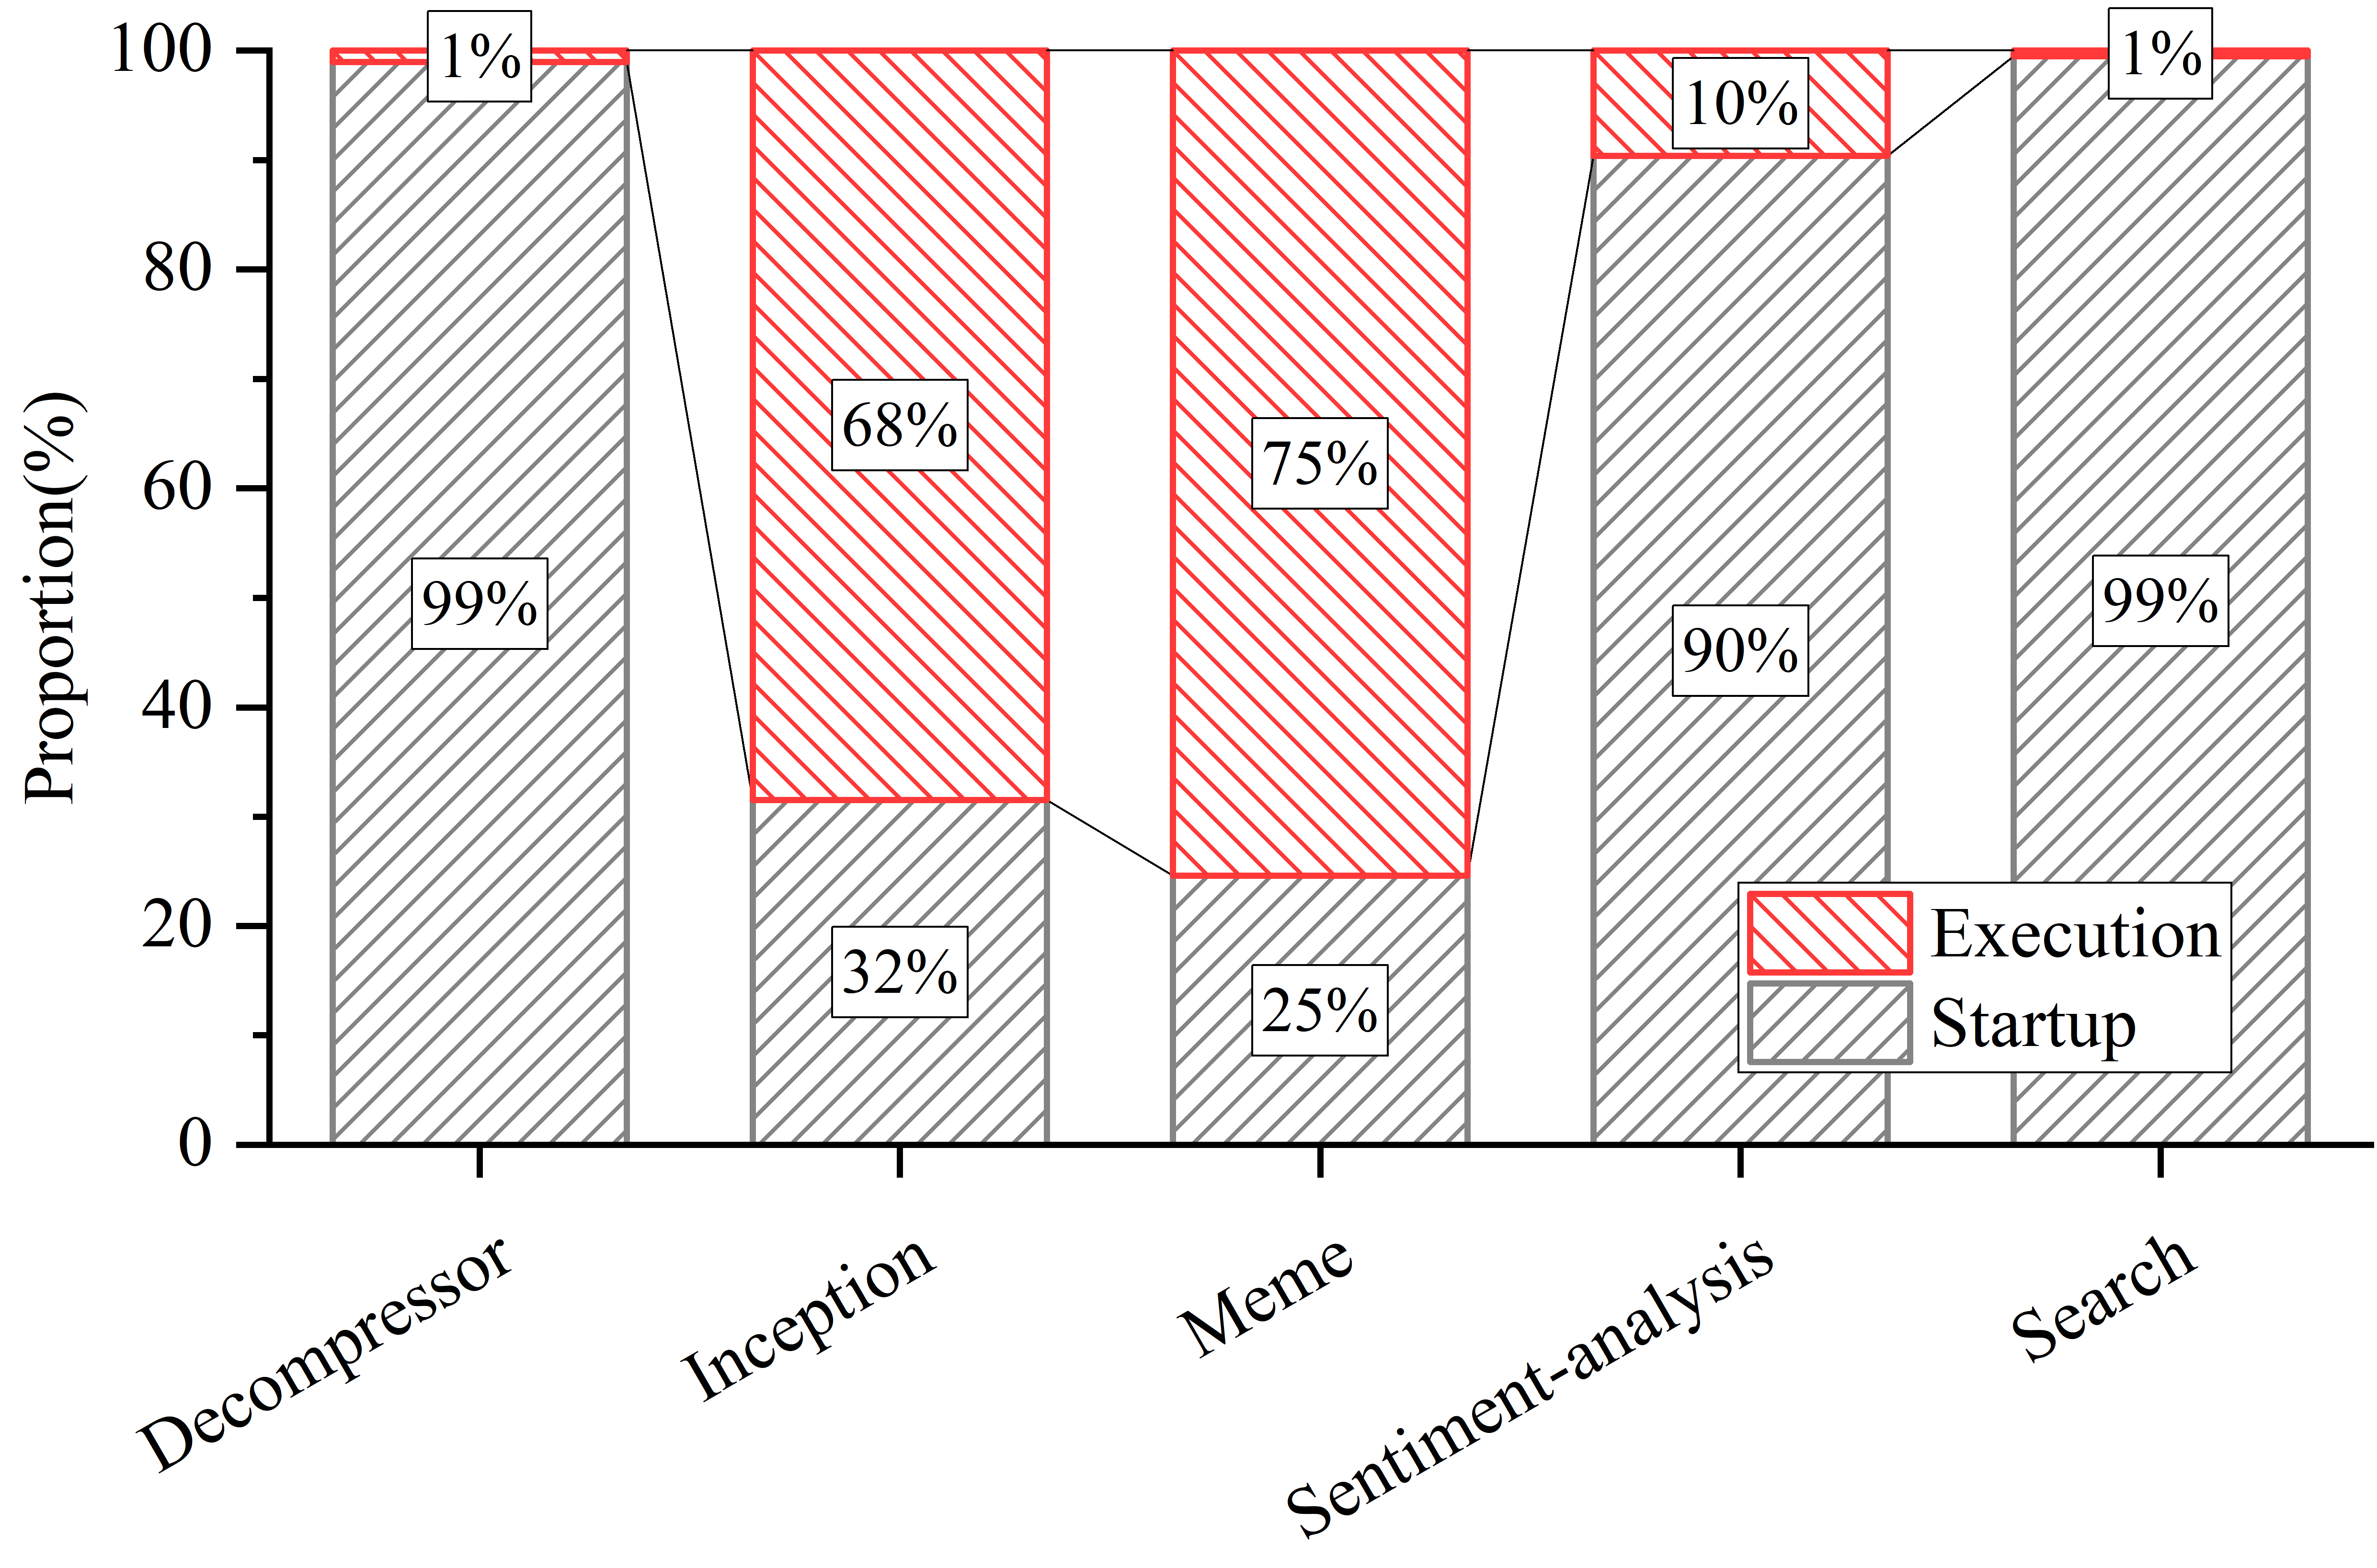
\includegraphics[width=3in]{images/default-proportion.png}
    \caption{Execution(and Startup)/Overall latency ratio of serverless functions.}
    \label{default-proportion}
\end{figure}

\begin{table}[htbp]
    \centering
    \caption{The Overall latency}
    \begin{tabular}{cc}
        \hline
        Type               & Time(ms) \\ \hline
        Decompressor       & 90       \\
        Inception          & 3035     \\
        Meme               & 1228     \\
        Sentiment-analysis & 320      \\
        Search             & 2149     \\ \hline
    \end{tabular}
    \label{overall-latency}
\end{table}

Minimizing the startup latency of serverless functions is critical to improving the user experience of the platform\cite{serverless-user-experience-1,serverless-user-experience-2},
and it is also one of the major challenges facing serverless computing\cite{berkeley-view,serverless-trends}.
Existing solutions reduce the response latency of the serverless computing platform by caching function instances\cite{pool1,pool2} or customizing the virtual environment of functions\cite{firecracker,faasm},
but these solutions cannot effectively reduce the initialization latency of the application.
Subsequent research shows that application initialization accounts for a large part of the function startup latency.


This paper proposes \textbf{ProjectName}, 
a design that effectively reduces the cold start latency of containerized serverless functions. 
\textbf{ProjectName} starts a function instance by restoring it from a checkpoint image and there by skip the initialization of serverless applications. 
Since the different functions of one serverless computing application have the same isolation state, 
we can achieve the purpose of boosting the initialization of the function sandbox by caching the isolation resources. 
At the same time, because functions typically access only a small fraction of memory at runtime, 
which allows us to enable on-demand loading of memory data through mapping strategy. 
Memory mapping also allows multiple functions to share read-only memory pages, 
which greatly reduces the memory footprint of functions in large-scale deployment scenarios.

We evaluate the performance based on open source application test sets and typical serverless computing applications developed in four programming languages.
The result shows that for all test cases, \textbf{ProjectName} can achieve <50ms startup latency, 
10x speedup over default startup strategy 
and 3x speedup over default restore strategy. 
\textbf{ProjectName} can also effectively reduce the memory footprint of 
functions by more than 90\%.

We believe our work makes the following contributions:

\begin{itemize}
    \item A detailed analysis of the containerized serverless function startup process.
    \item Several optimisation on the function restoring process to further improve the cold start efficiency of functions.
    \item Experiments based on multiple types of serverless applications proving the effectiveness of our system.
\end{itemize}


The remaining sections are structured as follows: 
Section II introduces the background and analyses the problem raised from serverless computing; 
Section III presents the core idea of \textbf{ProjectName}; 
Section IV shows the experimental results and Section V discusses the related work; 
Section VI conclude our work and future directions.
\section{background}

In the Function-as-a-Service(FaaS)\cite{berkeley-view} incarnation of the serverless model,
the smallest unit of calculation used is a serverless function written by the user.
When the serverless computing platform receives a service request or a predefined event is triggered,
the serverless computing platform will initialize a temporary execution sandbox(containers\cite{container-in-serverless-1,container-in-serverless-2} or virtual machines\cite{firecracker,vm-in-serverless-1}, etc.),
and run the function uploaded by the user in the sandbox to process the request. After the execution, the sandbox will be destroyed,
and the occupied resources will be recycled for the next request.

The serverless function goes through three stages(as shown in the figure \ref{startup-periods}) when it starts.
The function isolation environment initialization stage refers to the creation and startup process of the sandbox(containers or virtual machines) for running serverless functions;
the runtime startup phase mainly refers to the initialization process of the function runtime, such as JVM and Python interpreter,
and the application startup phase mainly refers to the startup process of the serverless application in the sandbox.

\begin{figure}[t]
    \centering
    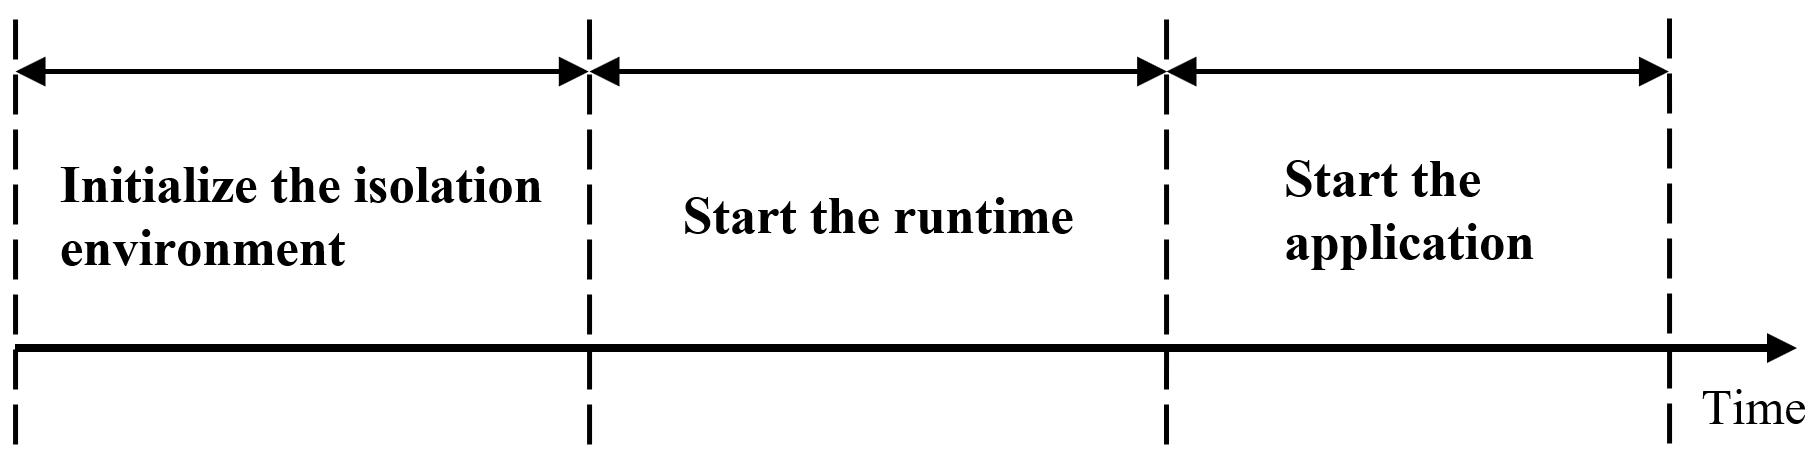
\includegraphics[width=\linewidth]{images/startup-periods.PNG}
    \caption{Startup process of a serverless function}
    \label{startup-periods}
\end{figure}

\subsection{Existing Startup Optimizations}

\subsubsection{Cache-based Optimizations}
Many systems\cite{pool1,pool2} adopt a pooling strategy to cache function instances.
When request come,
a pre-warmed function instance is taken out from the pool to handle the request,
thereby improving the execution performance of the system.
Although the cache-based strategies can greatly reduce the response latency of serverless computing platforms,
it also reduces the resource utilization of the system and increases costs.
At the same time, it brings great difficulties to the elastic scaling of function instances.

\subsubsection{Isolation Sandbox Optimizations}
By optimizing the isolation sandbox of serverless functions,
the startup performance of the function can be improved.
For example,
FAASM\cite{faasm} introduces the SFI mechanism used in WebAssembly to isolate the memory space of serverless functions.
SFI allows multiple serverless functions to share memory resources while isolating memory.
For the limiting of other resources(such as CPU and network), FAASM uses standard Linux cgroups.
FAASM also provides a low-level POSIX interface for isolated serverless functions to operate on the network and filesystem.
gVisor\cite{gvisor} is a new type of sandbox technology released by Google,
which is essentially a system kernel written in Go language and running in user mode.
Depending on its configuration,
gVisor can use the corresponding mechanism provided by ptrace or KVM to intercept the system calls of the application,
and act as a guest kernel to provide services for the application without using hardware virtualization.
Such a design can bring lower resource consumption,
while reducing the cost of virtualization,
thereby bringing better startup performance.
For most serverless computing applications,
the runtime startup and application startup latency account for a large part. The method of simplifying the isolation environment cannot effectively optimize these stages,
so the overall startup latency is still considerable.

\subsubsection{Checkpoint/Restore-based Optimizations}
SEUSS\cite{seuss}, Catalyz\-er\cite{catalyzer}, Prebaking\cite{prebaking} and other systems use checkpoint technique to create checkpoints on running functions.
By restoring from an existing function checkpoint,
the runtime startup latency and the application startup latency of the function can be effectively reduced.
At the same time,
Catalyzer also optimized the function restore process to further improve the efficiency of function startup.
SEUSS, Catalyzer uses a customized operating system
or modifies the language runtime to achieve the best performance,
but it also brings compatibility issues,
making the system difficult to maintain and manage.
Prebacking restores containerized serverless functions based on the C/S technique provided by CRIU\cite{criu},
but the acceleration mechanism based on restoration still has room for further optimization.
To illustrate this problem,
we use the existing C/S mechanism to restore the function,
as shown in Figure\ref{default-restore} is the restoration latency of some typical serverless functions.

\begin{figure}[t]
    \centering
    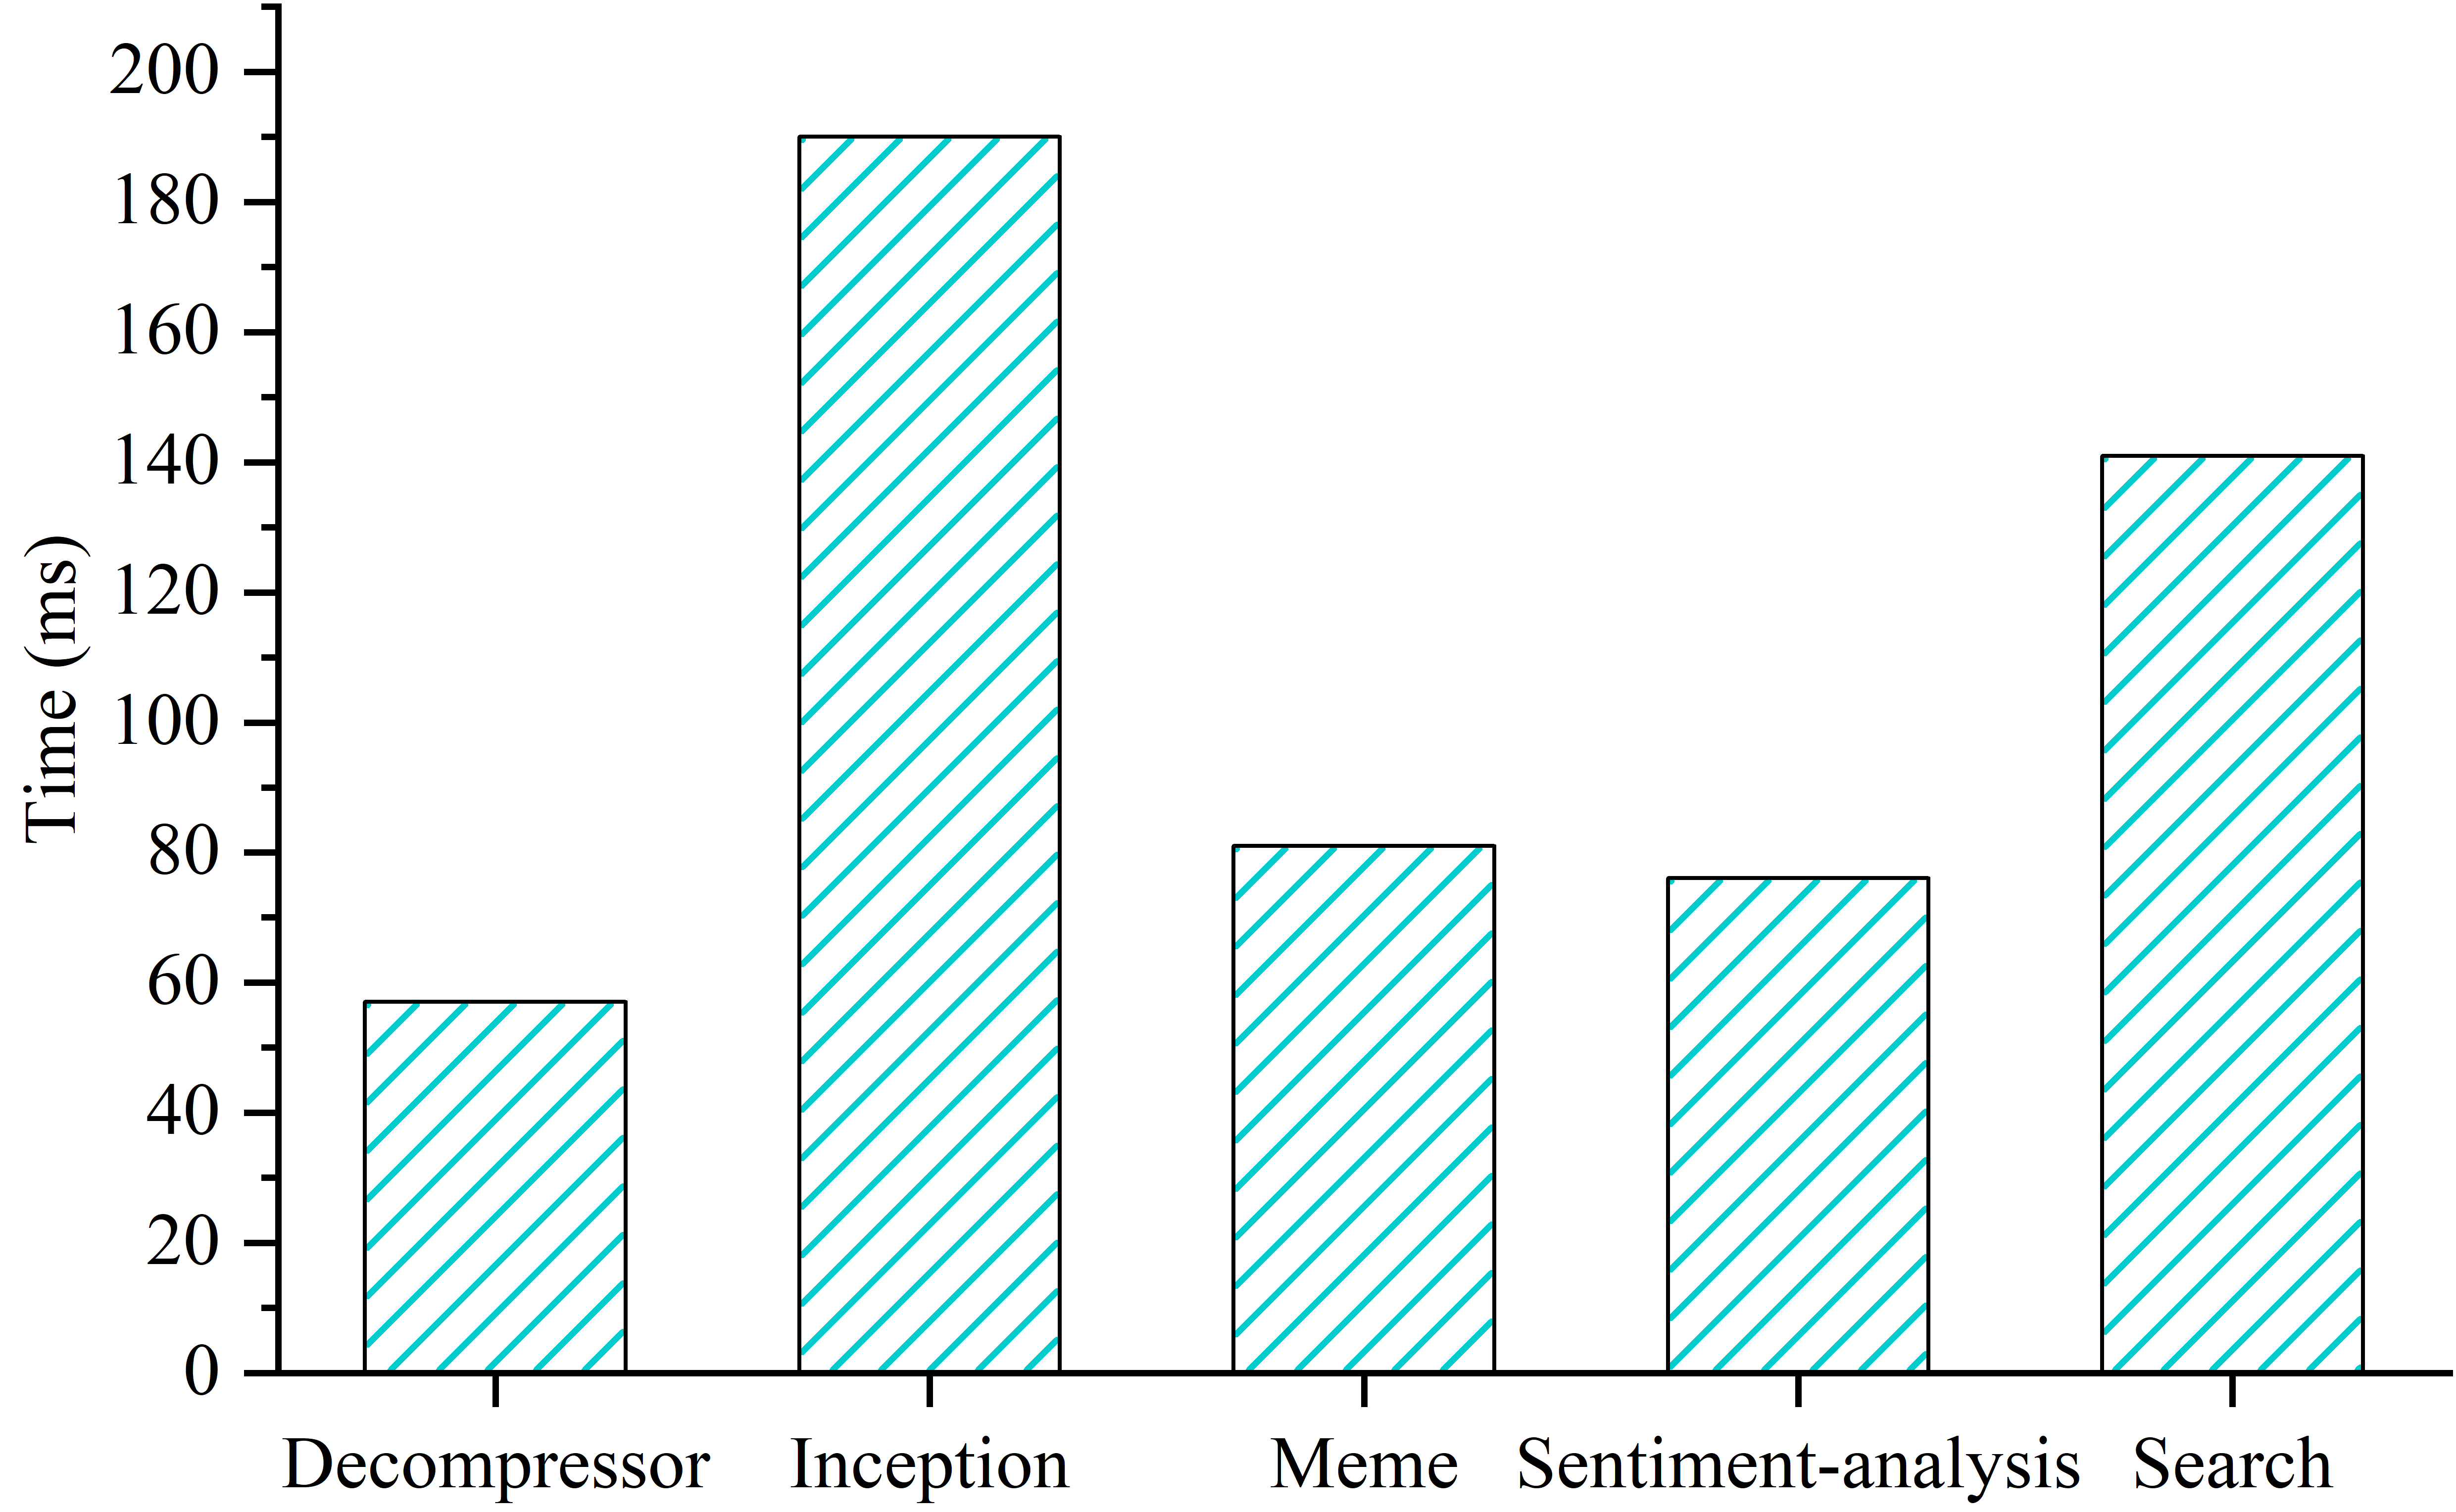
\includegraphics[width=3in]{images/default-restore.png}
    \caption{Restoration latency of serverless functions}
    \label{default-restore}
\end{figure}

Even if the C/S technique is used, some serverless functions still have considerable startup latency,
and the startup latency of functions has great volatility due to the complexity of different applications.
There is another issue worth noting—resource usage.
The figure \ref{restore-mem} is the memory usage of different serverless functions after 10 startups.
Due to the completely independent memory space between each function process,
it causes extreme large resource consumption,
which is not conducive to the large-scale deployment of serverless functions.

\begin{figure}[t]
    \centering
    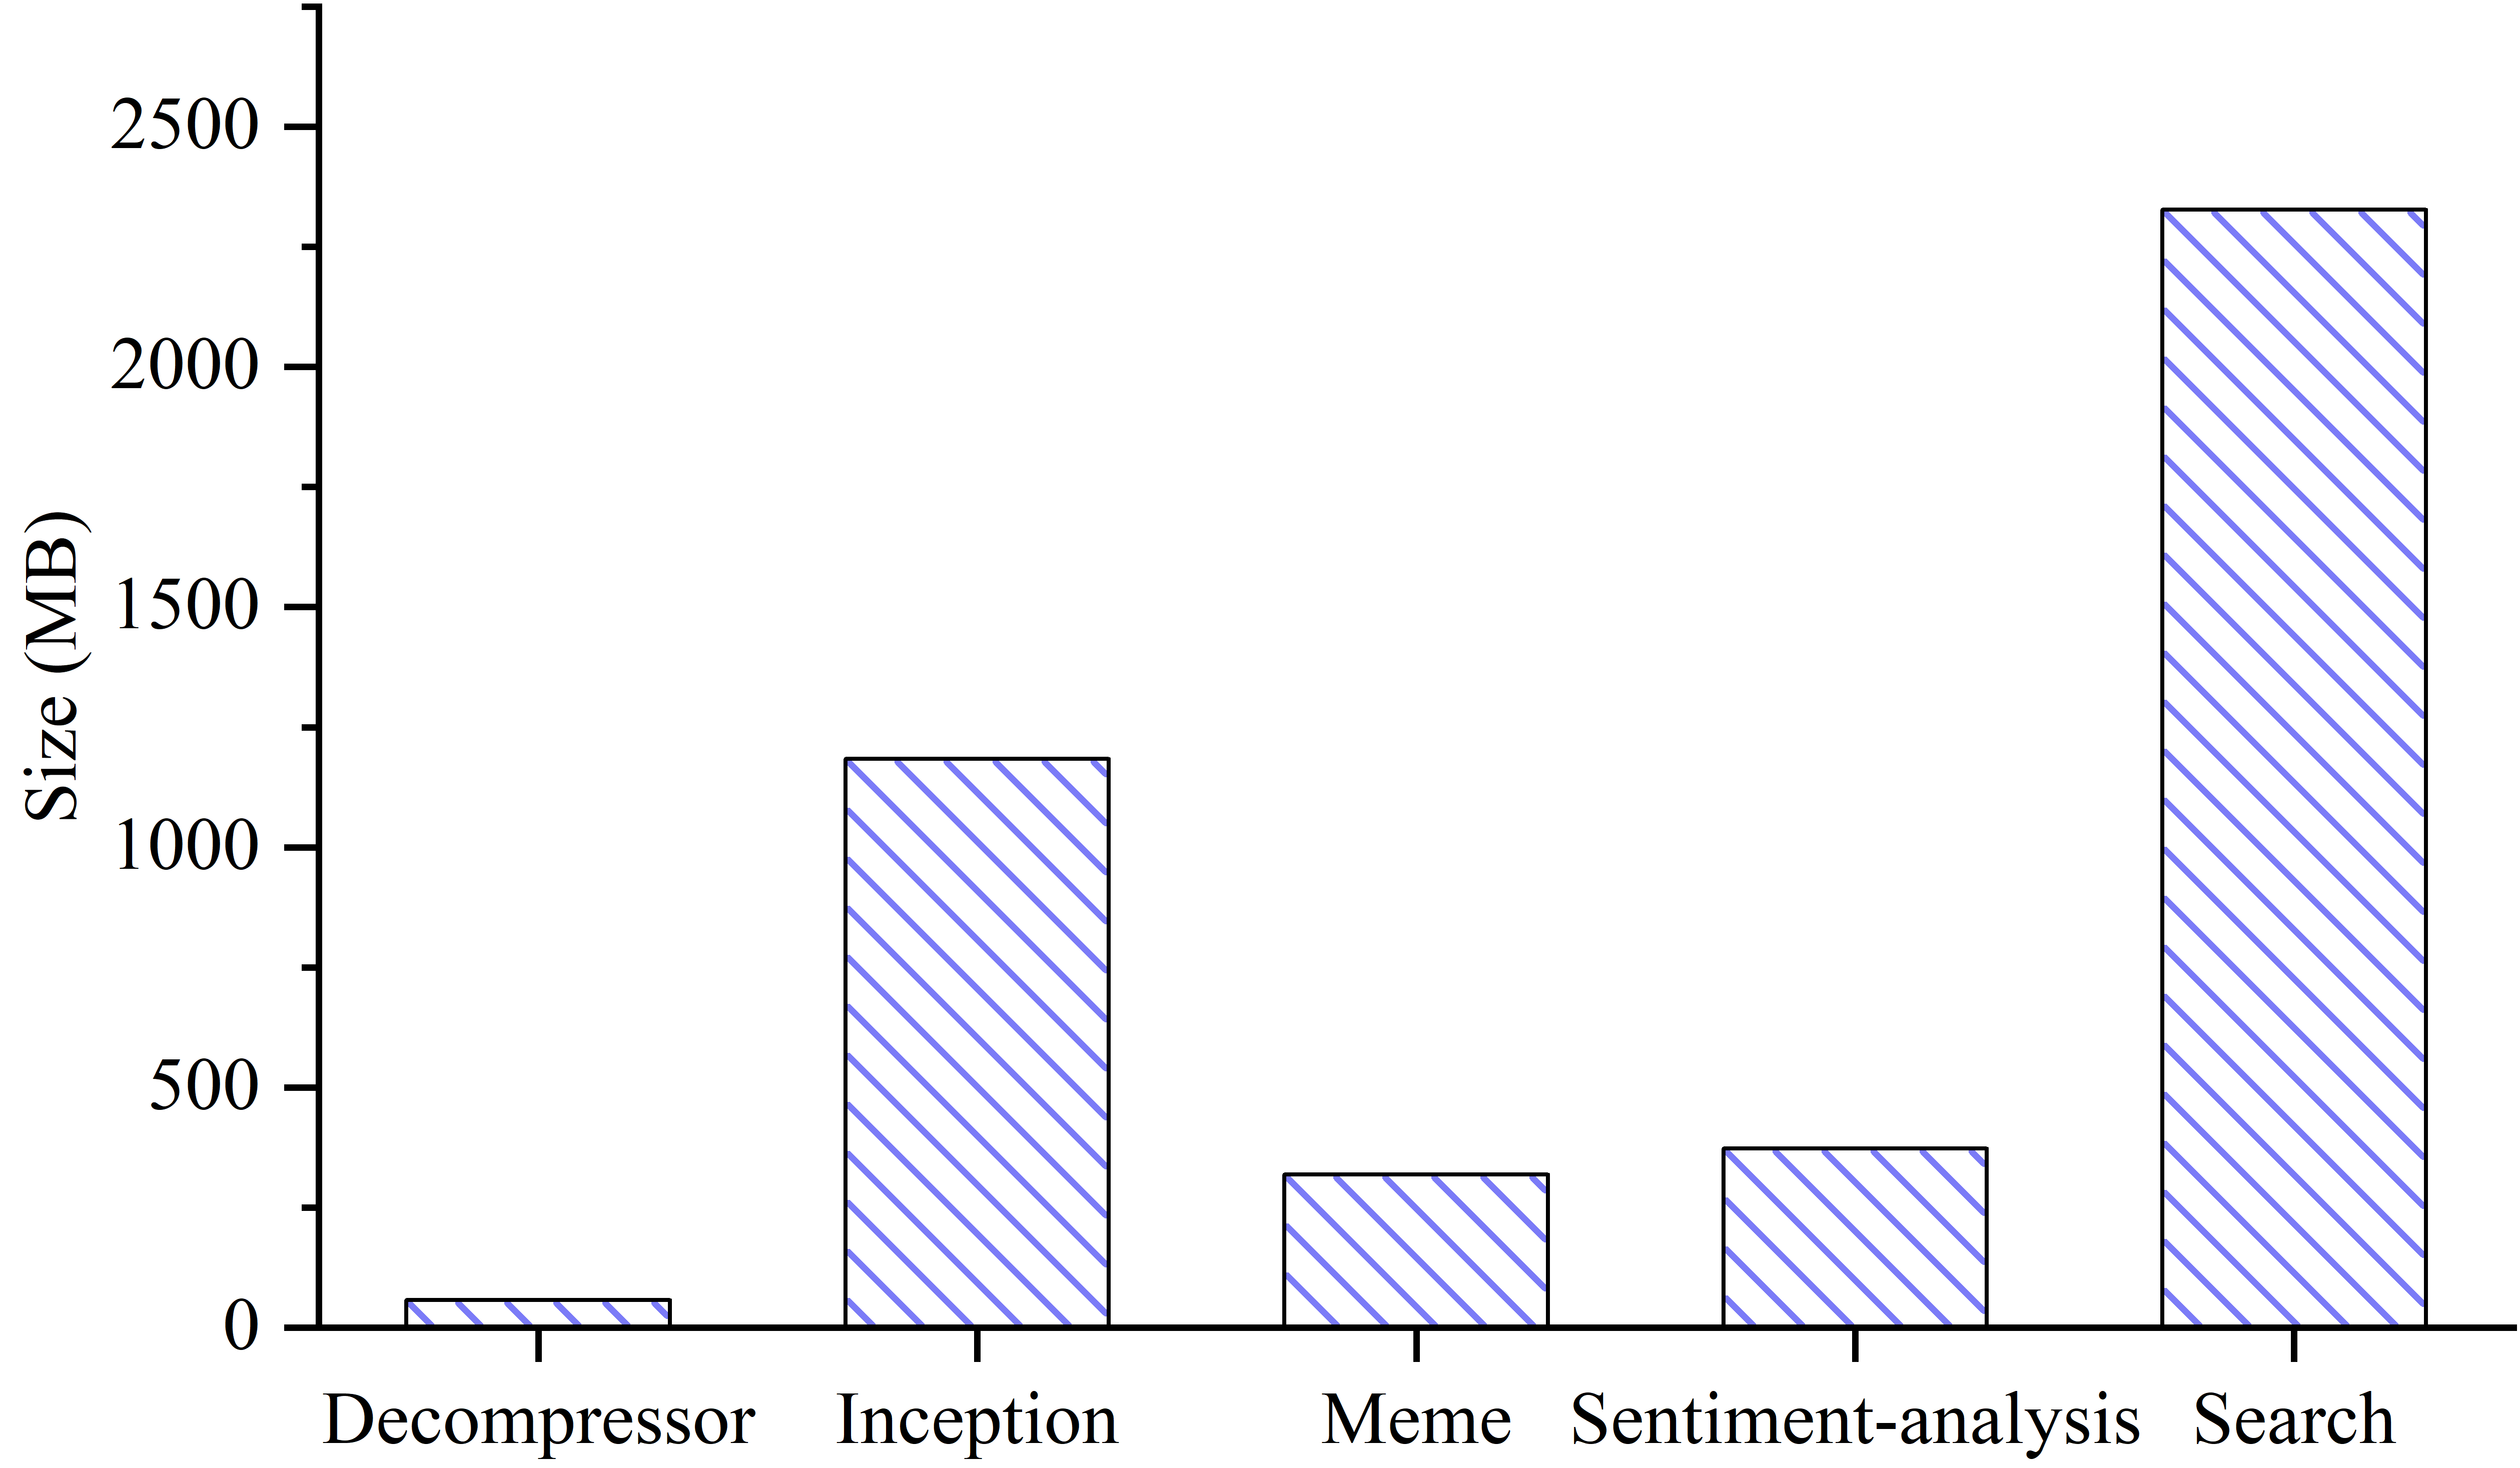
\includegraphics[width=3in]{images/default-resotre-mem.png}
    \caption{Memory usage of serverless functions after 10 starts}
    \label{restore-mem}
\end{figure}

\subsection{Analysis of Serverless Function Restoring Process}


\begin{figure*}[t]
    \centering
    \subfigure[\label{golang-restore}A Golang-based function]{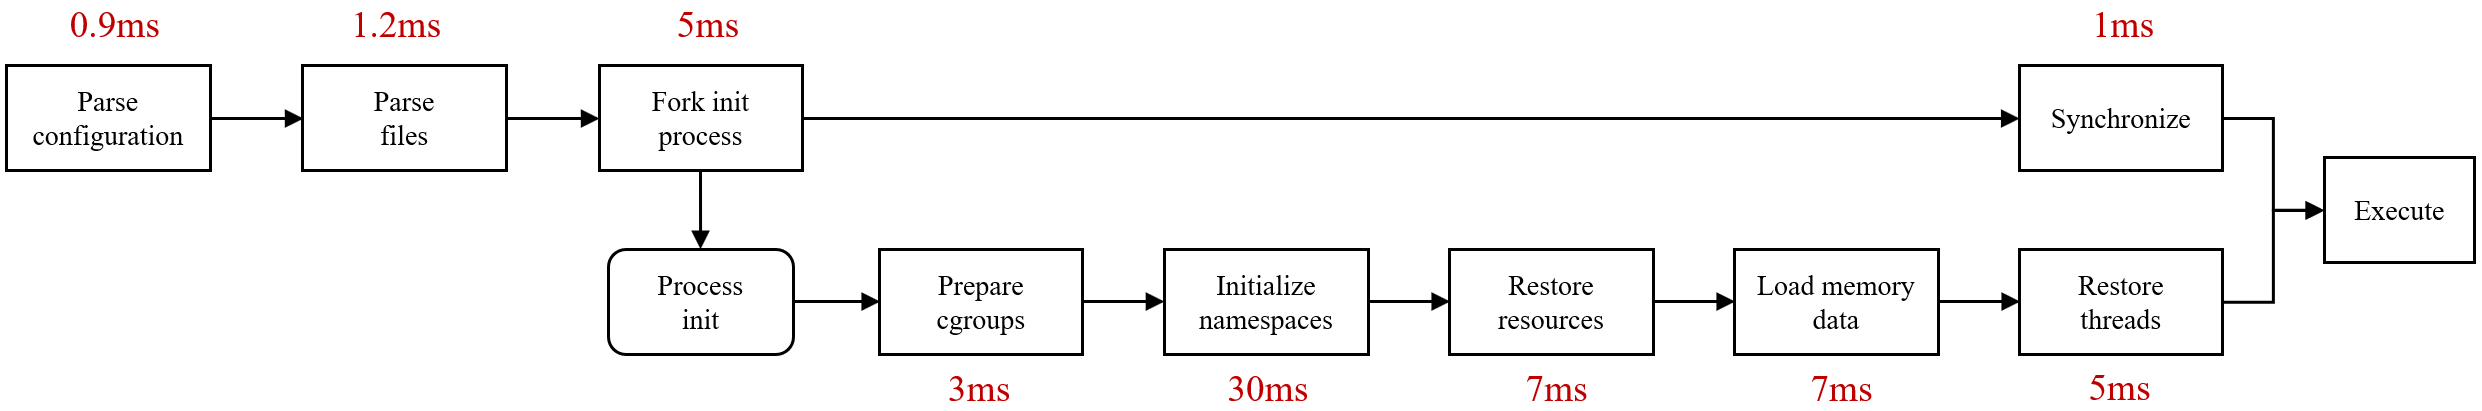
\includegraphics[width=6.5in]{images/golang-restore.PNG}}
    \subfigure[\label{java-restore}A Java-based function]{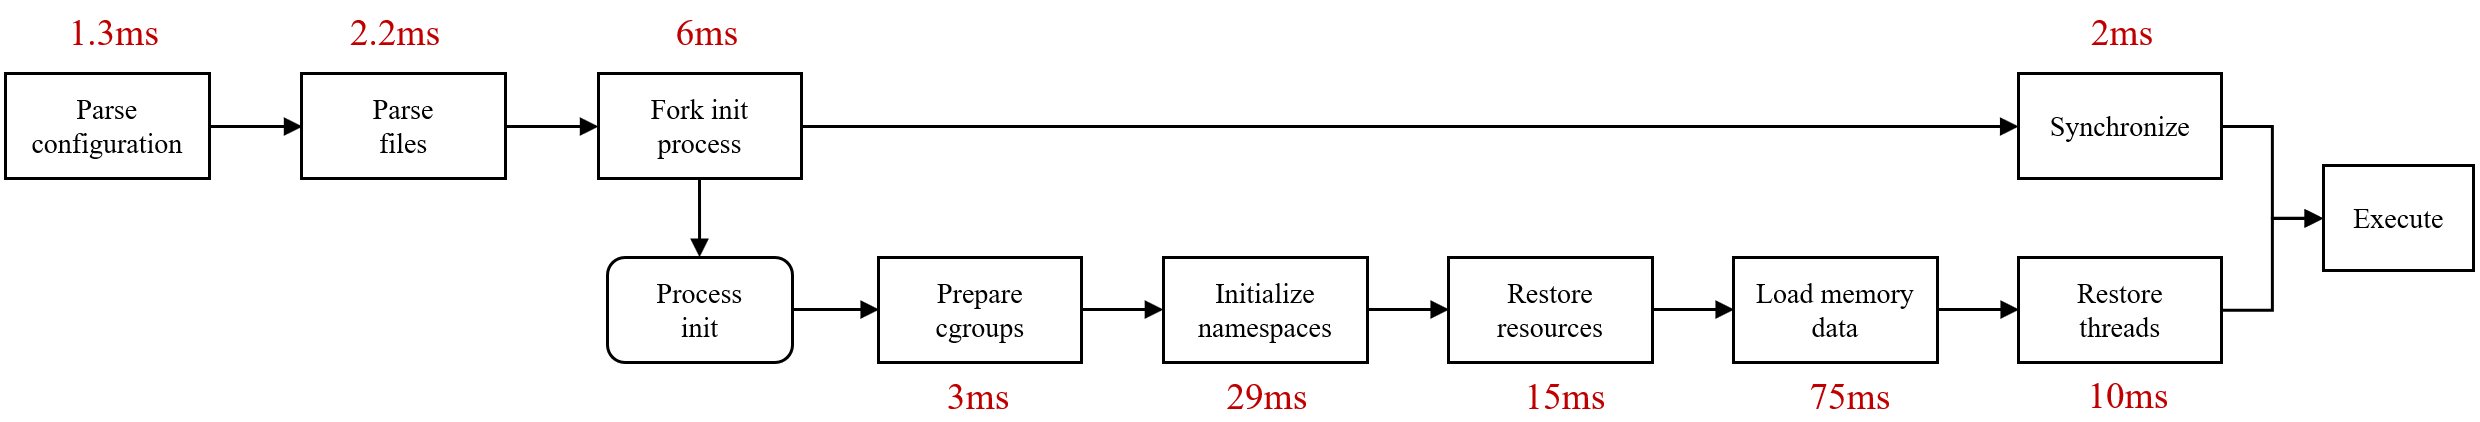
\includegraphics[width=6.5in]{images/java-restore.PNG}}
    \caption{Restoration process of serverless functions}
    \label{restore-process}
\end{figure*}

The containerized serverless function will go through multiple stages as shown in the figure\ref{restore-process} during recovery,
which mainly include configuration analysis,
init process creation,
isolation environment initialization,
resource restoration,
memory data loading,
thread restoration, etc.

In the namespace initialization stage,
CRIU will create multiple brand new namespaces,
and then configure these namespaces according to the contents of the checkpoint.
For example,
for Mount namespace,
CRIU mounts filesystems and devices according to the relevant information from the checkpoint, and for IPC namespace,
CRIU restores Linux system V IPC items.
These additional restoration work brings a fixed and considerable delay to the start of the function.
However, in the memory loading stage,
CRIU copies all memory data to the memory space of the function process,
because different serverless functions have different memory footprints,
the delay in this stage varies.
For example,
Java-based serverless functions(figure \ref{java-restore}) have higher memory loading latency than Golang-based(figure \ref{golang-restore}) functions. 
The way of copying makes multiple function processes have independent memory data, 
resulting in data redundancy.

\textbf{Difficulties in optimization.} Although the initilization of the isolation environment can be optimized by simply simplifying the isolation environment, 
it will reduce the isolation strength and the security of the container. 
At the same time, memory data is necessary for the running of the function, and this stage cannot be optimized by omitting data transmission. 
Therefore, 
the main difficulty lies in how to combine the characteristics of the container environment to speed up the initialization process of the sandbox, 
while adopting an appropriate method to reduce the amount of memory data read during the function startup process, 
improve the initialization efficiency and ensure the correctness of the function.
\section{Design}

\begin{figure}[t]
    \centering
    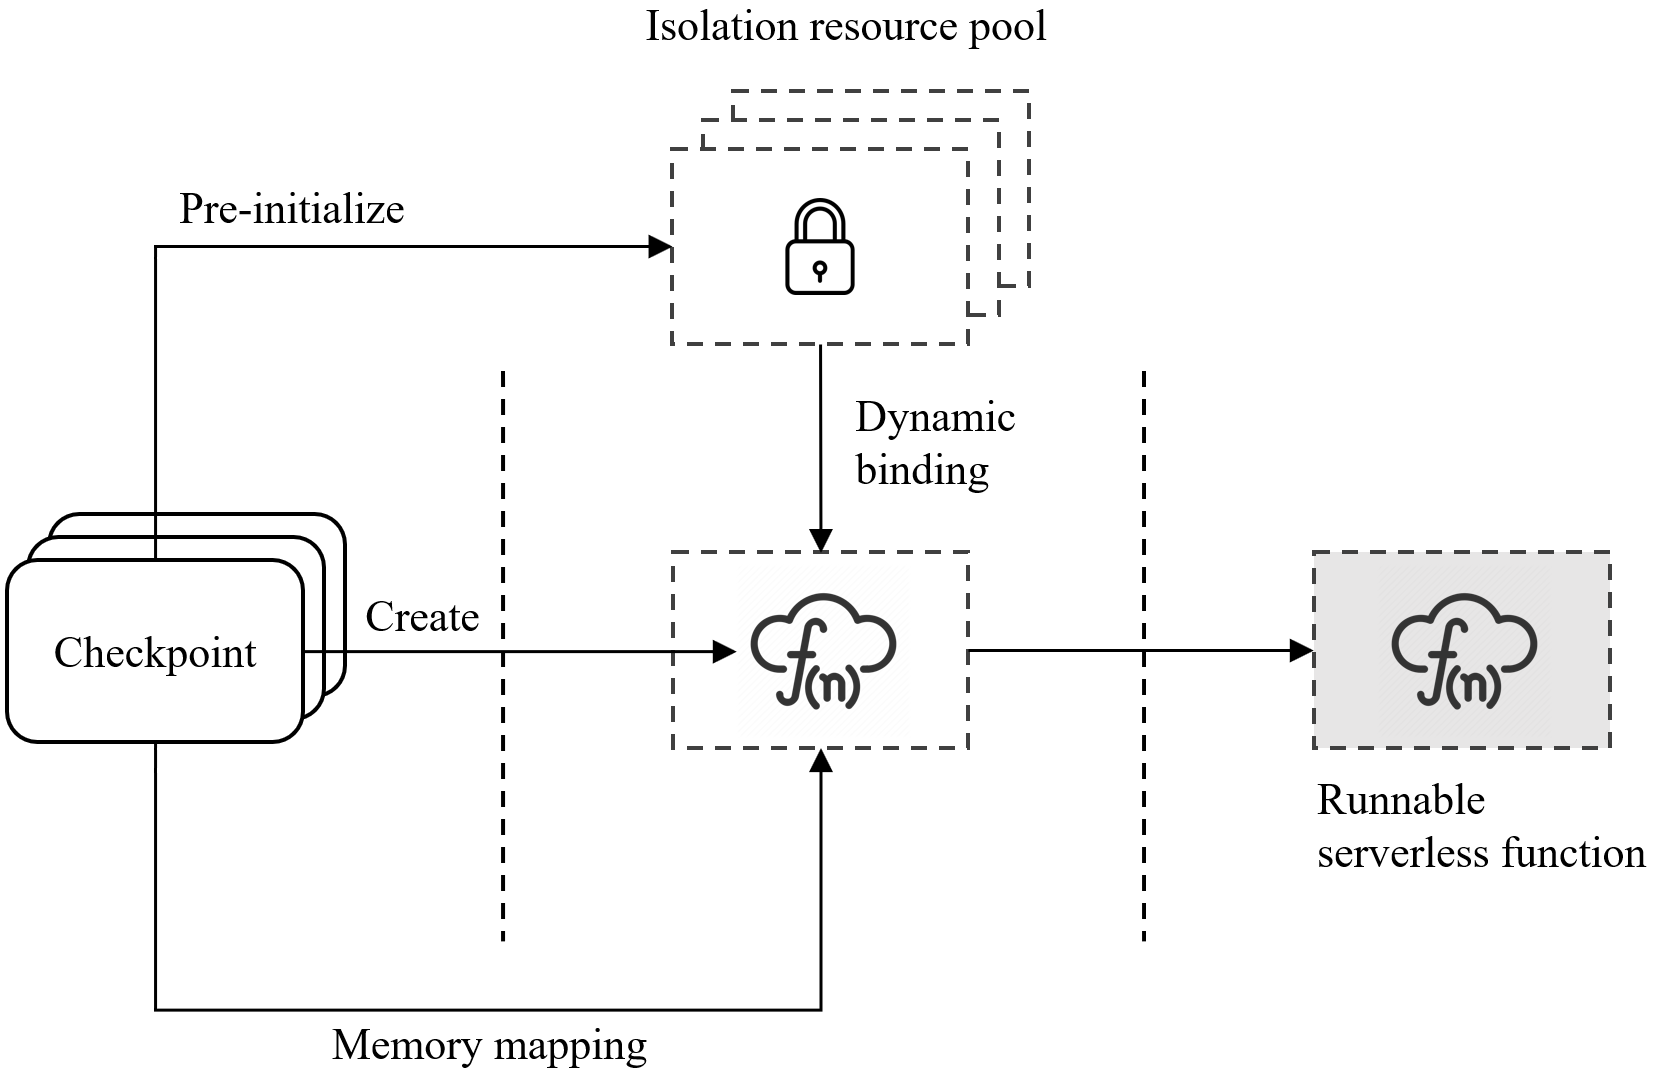
\includegraphics[width=\linewidth]{images/design.PNG}
    \caption{Overview of ProjectName}
    \label{design}
\end{figure}

In this paper we propose \pname, 
which is mainly based on CRIU, 
and uses multiple optimization mechanisms to effectively reduce the complexity of the restoration process of serverless functions, 
providing a stable and better startup performance.


As shown in the figure \ref{design}, 
before starting the function, 
\pname will use the information recorded in the function checkpoint to \textit{pre-initialize} 
multiple namespace resources required to build the sandbox environment, 
which constitutes the \textit{isolated resource pool}.
When \pname receives the request to start the function and creates the function process, 
it will \textit{dynamically bind} the function process and the matching namespace resource to speed up the construction of the sandbox environment. 
Then \pname restores the function memory data through \textit{memory mapping}, 
and finally produces a \textit{runnable serverless function}.

\subsection{Isolation Environment Pooling}
Since the Linux namespace can exist independently of the process, 
that is, 
as long as the file descriptor of the corresponding namespace is opened or bind-mounted to another location, 
even if the process inside the namespace exits, 
the namespace is still valid, 
and other processes can use system calls such as setns to enter the namespace and modify the related resources referenced by it. 
Based on this feature, we propose an isolation environment pooling strategy for the construction of the function isolation environment.

The strategy creates multiple brand new Mount, UTS, and IPC namespaces in the system before the serverless function starts. 
The newly created namespace cannot be used to assemble the serverless function. Therefore, the strategy needs to parse the checkpoint of each serverless function and initialize each namespace according to the information inside the checkpoint. 
For example, for Mount namespace, 
the function checkpoint contains the mounting information of each filesystem and device in the namespace. 
Using information from the checkpoint, 
the pooling strategy will mount the corresponding filesystem or device to the correct directory location through the recorded mounting parameters; 
for UTS namespace, 
The pooling strategy sets the correct host name and domain name of the container; 
for the IPC namespace, 
relevant core parameters are set  
and structures such as shared memory, 
message queues, and semaphores are created and initialized. 
Through this strategy, 
CRIU does not need to initial Mount, UTS, and IPC namespace again when starting the serverless function, 
but only needs to enter the prepared isolation environment through the setns system call. 

The isolation environment pooling strategy 
essentially removes the function isolation environment 
initialization phase from the startup process and places it to the offline, 
which can greatly reduce the latency in the isolation environment 
initialization phase under the premise of extremely low resource consumption. However, 
this scheme has certain security risks. 
Because the \textit{/proc} directory of the root filesystem provided by the container is attached by the \textit{proc filesystem}, at the same time, 
multiple subdirectories under the \textit{/proc} directory are read-only bind-mounted to prevent the container process from modifying the contents of the directory, which ensures the security of the host. 
The contents of the files and directories contained in the \textit{proc filesystem} are directly related to the PID namespace of the process that mount the \textit{proc filesystem}. 
For example, 
the \textit{/proc/[pid]} subdirectories in the \textit{proc filesystem} only expose the information of all processes in the same PID namespace. 
If the isolation environment pooling strategy is adopted, 
the Mount namespace used by the serverless function will be initialized, 
and the component or system that implements the strategy will use a process to 
attach \textit{/proc} directory with \textit{proc filesystem}, 
which causes the inconsistency between the process that mount the \textit{proc filesystem} and the process ultimately running in this namespace. 
If the function process use the pre-initialized Mount namespace directly, 
it will bring security risks of host data leakage, 
which may cause the function to exit, 
or damage the security of the container environment.

\begin{figure}[t]
    \centering
    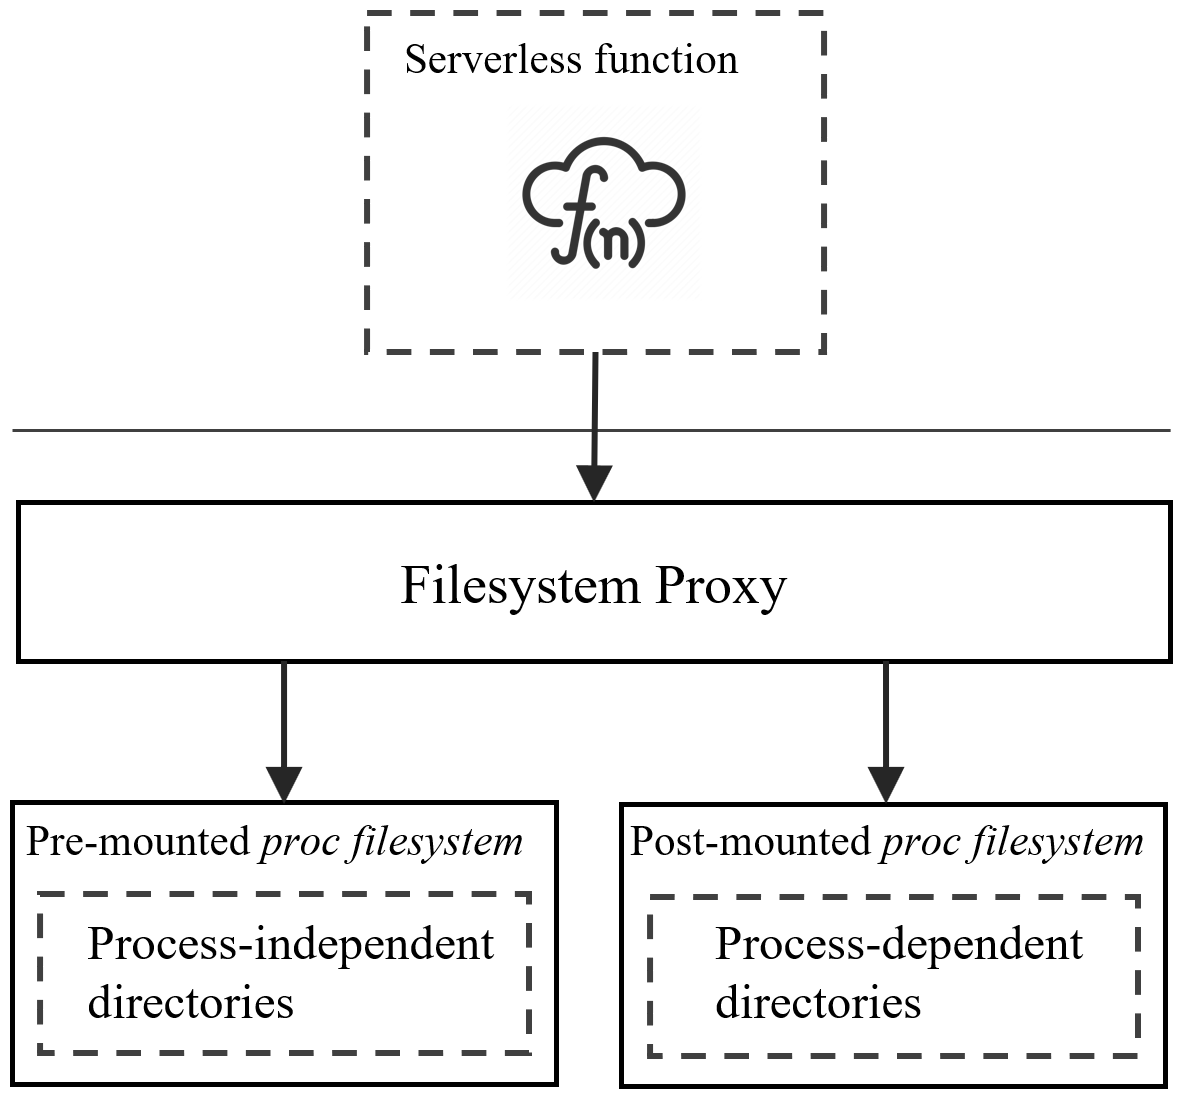
\includegraphics[width=2.5in]{images/fs-proxy.PNG}
    \caption{Filesystem proxy}
    \label{fs-proxy}
\end{figure}
In order to avoid the introduction of the aforementioned systemic risks and ensure the efficiency of function startup, 
\pname introduces the \textit{filesystem proxy} 
which forwards requests from processes in the container to access the /proc directory. 
As shown in the figure \ref{fs-proxy}, 
There are two types of \textit{proc filesystem} below the \textit{filesystem proxy}. 
One is the \textit{"pre-mounted proc filesystem"} which is mounted through the isolation environment pooling strategy, 
the other is the \textit{"post-mounted proc filesystem"} that is simply mounted by the container process when the container starts. 
When a serverless function accesses the \textit{/proc} directory, 
it will first access the \textit{filesystem proxy} layer. 
The \textit{filesystem proxy} will judge the specific directory to be accessed. 
If the directory to be accessed containes content that has nothing to do with the process PID namespace, 
the access request will be forward to the \textit{"pre-mounted filesystem"}, 
otherwise the \textit{filesystem proxy} will synthesize the contents of the corresponding directory of the \textit{"post-mounted proc filesystem"} 
and the access attributes of the corresponding directory of the \textit{"pre-mounted proc filesystem"} to give a correct response. 
Using the \textit{filesystem proxy strategy} to forward access requests not only ensures the effectiveness of the pooling strategy, 
but also prevents the security of the container environment from being weakened.

\subsection{Function Memory Shared Mapping}
\begin{figure}[t]
    \centering
    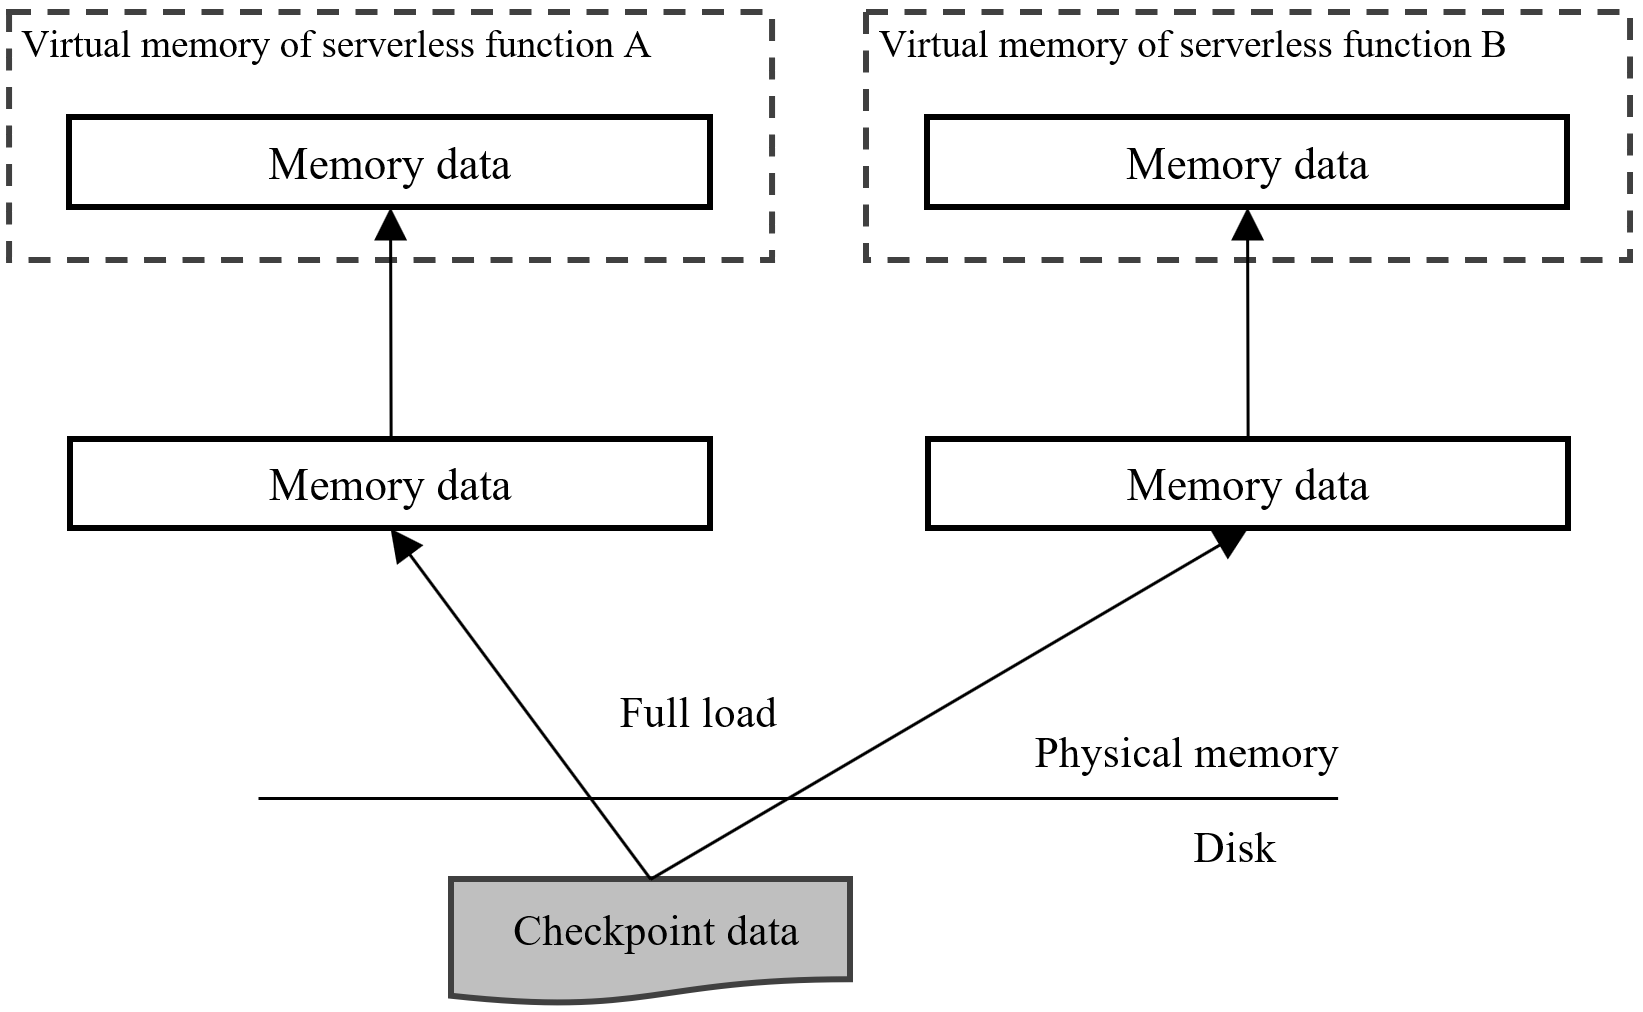
\includegraphics[width=\linewidth]{images/full-load-memory.PNG}
    \caption{Memory data redundancy brought by multiple identical serverless functions}
    \label{full-load-memory}
\end{figure}

As shown in the figure \ref{full-load-memory}, 
CRIU uses a full-load method when restoring the function memory data, 
which copies the memory page data from the checkpoint to the corresponding location in the process's virtual memory space. 
For serverless functions that require a large amount of memory in runtime, the checkpoint contains more memory data. 
Since the reading of the checkpoint is essentially a reading to the disk, 
it brings quite high latency. 
At the same time, 
the full-load method results in multiple copies of the same data in the physical memory. 
Even if the memory data of multiple identical serverless functions are basically the same, 
because the memory data cannot be shared between function processes, 
memory data redundancy occurs, 
which severely reduces the resource utilization of the platform.

\begin{figure}[t]
    \centering
    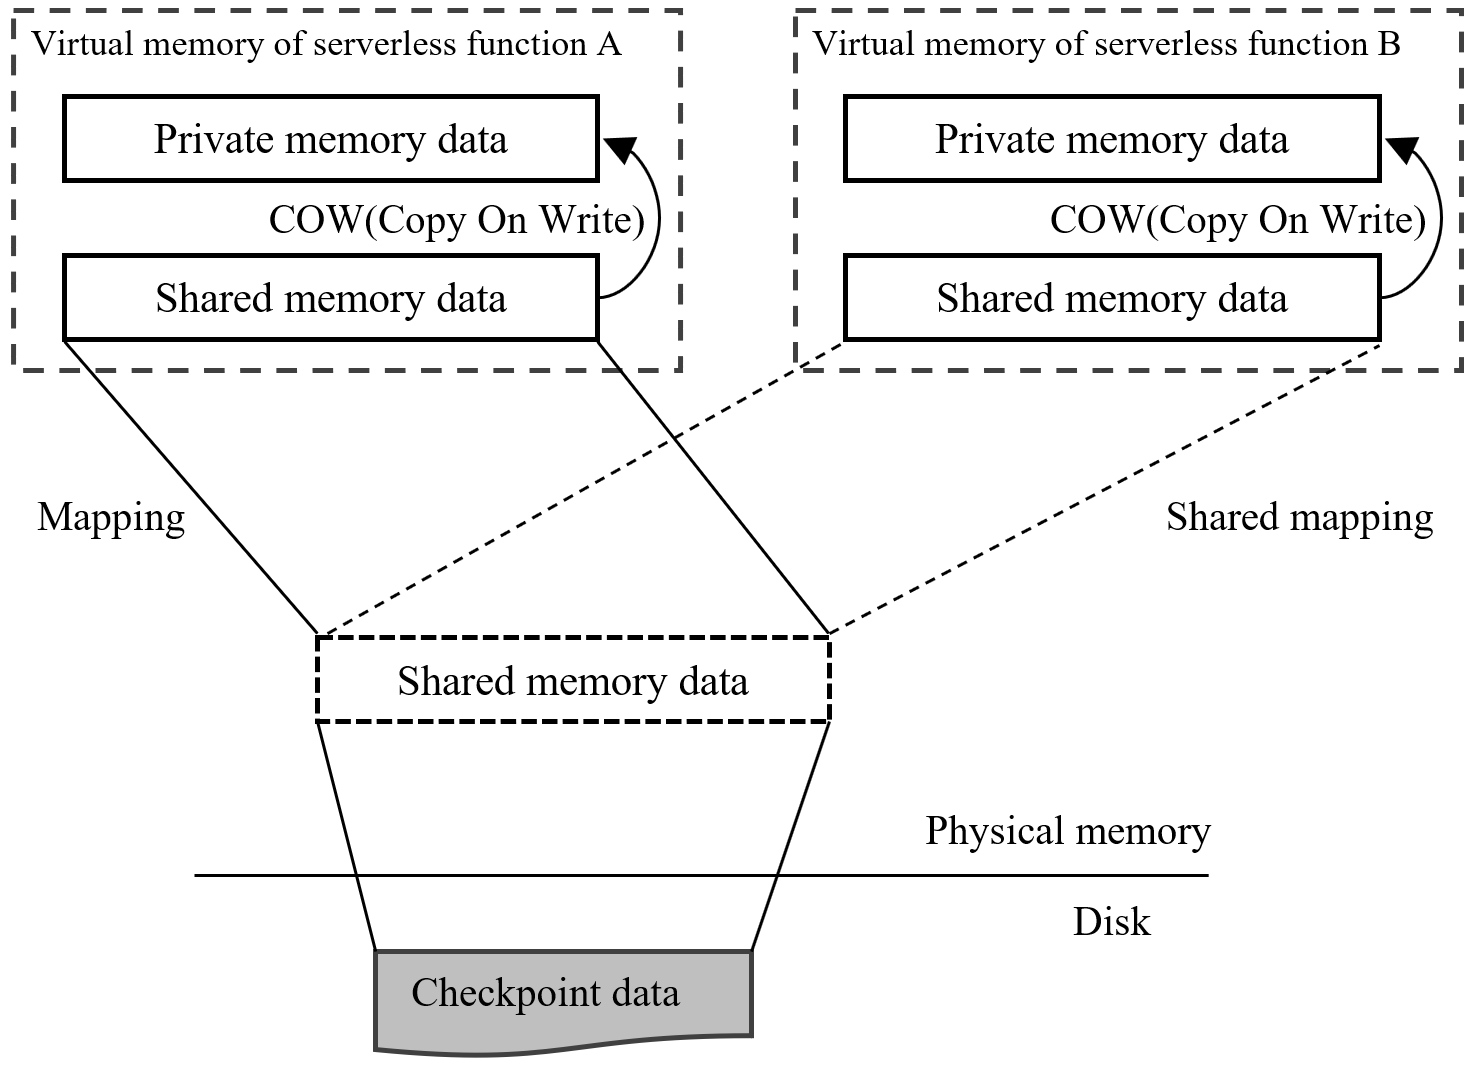
\includegraphics[width=\linewidth]{images/shared-memory.PNG}
    \caption{Function memory shared mapping}
    \label{shared-mapping}
\end{figure}

This paper introduces the shared mapping strategy 
of function's memory to replace the original memory restoration method of CRIU. 
As shown in the figure \ref{shared-mapping}, 
the CRIU restores the memory data of serverless functions by 
establishing the mapping relationship between the virtual memory space 
of the function process and the corresponding memory page in the checkpoint. 
This mapping does not lead to the reading of the memory data. 
Only when the serverless function accesses the mapped virtual memory space during the startup, 
the corresponding data in the checkpoint will be loaded into the physical memory.
This memory restoration method allows the memory data in the checkpoint to be loaded into the physical memory on demand, which greatly reduces the delay of the restoration of the memory data, and avoids temporarily unnecessary data from being copied to the physical memory prematurely, 
causing a waste of system resources.

At the same time, 
the mapping method allows multiple serverless 
functions started from the same checkpoint to share the same physical memory space, 
avoiding the waste of resources when a serverless computing application is deployed on a node on a large scale. 
As shown in the figure \ref{shared-mapping}, 
the memory pages mapped into the virtual memory space of the function process are all read-only. 
When the function process tries to modify the data of a certain memory page, 
the \textit{Copy on Write(COW)} mechanism of the operating system  
will make a copy of the page for private write operations.
\section{Implementation}

\pname is implemented based on containerd, runc and CRIU. 
These components have been extended to support the optimized startup of serverless functions. 
At the same time, the system also introduce the \textit{serverless function resources management component} to manage function namespace resources and checkpoint resources.

\subsection{containerd}
This system expands the original function startup process and function life cycle management logic of containerd. 
The extended containerd will use the packaged client to interact with the serverless 
function resource management component before starting the function. 
Containerd calls the service interface of resource management component passes 
in the function name and the required resource type, 
such as the namespace resource type or the checkpoint resource type. For the namespace resource type, 
it also needs to specify the detailed type of the namespace, 
such as Mount, IPC or UTS. 
After the call is successful, 
the serverless function resource management component 
will return the path and ID information of 
the corresponding resource, 
and containerd will record this information 
in the description file of the function to be started. 
The modified function life cycle management logic calls the corresponding interface of the function resource management 
component according to the resource information recorded in 
the description file after the function execution is completed, 
and returns the used resources.

\subsection{runc}

\pname has minor changes to runc. 
The extended runc component will convert the relevant resource information passed by 
containerd into a form that can be recognized by CRIU before calling CRIU to start the function process.

\subsection{CRIU}
When CRIU is started, 
it will determine whether there is the Linux namespace path information passed from runc in the startup parameters. 
If it exists, 
CRIU will directly use the setns system call to enter the namespace during the initialization of the namespace. 
At the same time, 
CRIU will determine whether the namespace type is Mount. 
If it is, CRIU also needs to setup the \textit{proxy filesystem}. 
The \textit{proxy filesystem} is implemented using FUSE\cite{fuse}, 
and CRIU mounts it to \textit{/proc} directory. 
Finally, when the CRIU initializes the memory data of the function process, 
it will calculate and record the offset position of the memory page data from the checkpoint in the virtual memory, 
and then use the mmap system call to map these pages to the virtual memory. 

\subsection{Serverless Function Resources Management Component}

As a resident service on the working node, 
this component implements the isolation environment pooling strategy and also manages the checkpoint of serverless functions. 
External services interact with this component through the packaged client library. 
There are two main back-end services of this component, 
the \textit{isolation environment resource management service} 
manages namespace resources for serverless functions 
and the \textit{checkpoint resource management service} manages
checkpoint resources of serverless functions.
When the \textit{isolation environment resource management service} starts, 
it will start multiple sub-processes based on the relevant information of the configuration file. 
These sub-processes will enter the new Linux namespace when they are created. 
The child process determines how to initialize 
the namespace by parsing the function checkpoint. 
For example, for Mount namespace, 
by parsing the checkpoint, 
the child process can obtain the type of filesystems 
that need to be mounted in the namespace. 
Subsequently, 
the child process will notify the main process of the resource management component 
to open the file descriptor corresponding to the initialized namespace 
to prevent the operating system from reclaiming the 
resources after the child process exits. 
At the same time, the component is also responsible for 
reinitializing the returned namespace resources. 
When the client requests the namespace of the function, 
the \textit{isolation environment resource management service} will return 
the path information of the corresponding namespace, 
that is, the corresponding path under the directory \textit{/proc/[pid]/fd/}. 

The \textit{function checkpoint resource management service}, 
manages the checkpoint of each function. 
it uses the containerd client to export the data of 
the function checkpoint for unified management when it is started.
\section{evaluation}

In this section, we evaluate the performance and scalability
of \pname against the \textit{Default-run}
(the default container startup method), \textit{Prebaking}\cite{prebaking}
(as a representative of unoptimized C/S-based container startup method)
and SEUSS\cite{seuss}.

\begin{table}
    \centering
    \caption{Test cases}
    \begin{tabular}{cccc}
        \hline
        Name               & Type                    & Language & Framework \\ \hline
        Text               & \makecell[c]{Text                              \\uploading}        & C++        & Thrift      \\
        Media              & \makecell[c]{Multimedia                        \\processing} & C++        & Thrift      \\
        ComposePost        & \makecell[c]{Database                          \\interaction}  & C++        & Thrift      \\
        UniqueID           & \makecell[c]{ID                                \\generating}         & C++        & Thrift      \\
        Timeline           & \makecell[c]{Timeline                          \\processing}   & C++        & Thrift      \\
        Decompressor       & \makecell[c]{Online                            \\decompressor}     & Golang     & Beego       \\
        Meme               & \makecell[c]{Image                             \\processing}        & JavaScript & Express     \\
        Inception          & \makecell[c]{Image                             \\classification}   & Python   & Flask       \\
        Sentiment-analysis & \makecell[c]{Sentiment                         \\analysis}      & Python   & Flask       \\
        Search             & \makecell[c]{Data                              \\retrieval}          & Java     & Spring boot \\ \hline
    \end{tabular}
    \label{table:test-case}
\end{table}

The serverless function test cases used in this section are shown in the table \ref{table:test-case}. 
Half of the test cases are derived from the \textit{Social Network} application in the 
microservice application set DeathStar\cite{deathstar}. 
The selected container service names are Text, Media, ComposePost, UniqueID, and Timeline; 
the other half of the test cases are serverless 
computing applications constructed in this paper based on different languages and development frameworks.

We use an x86-64 machine (the experimental machine) with 
an 8-core Intel i7-9700 CPU, 128GB memory and Samsung
1TB SSD, to evaluate our system. 
The OS is Ubuntu 18.04 with Linux kernel 5.8.9.

The experiment in this section is divided into three parts. 
The first part mainly verifies the optimization 
effect of our system in terms of serverless function startup latency. 
The verification method is to use all the systems under test 
to start multiple different types of serverless functions and record the function startup latency. 
The experiment will be performed multiple times to obtain the average startup latency of the function.
The second part of the experiment verifies the optimization effect of this system on the memory occupancy during deployment of serverless functions. 
The experiment use systems to start a certain number of serverless functions in each test cycle, 
wait for all functions to start and use related tools to record the memory usage of all functions. 
The third part of the experiment is to test 
the concurrent function deployment performance of the system. 
The verification method is to perform large-scale 
concurrent deployment of serverless functions on the experimental node.

\subsection{Function Startup Latency}

\begin{figure*}[t]
    \centering
    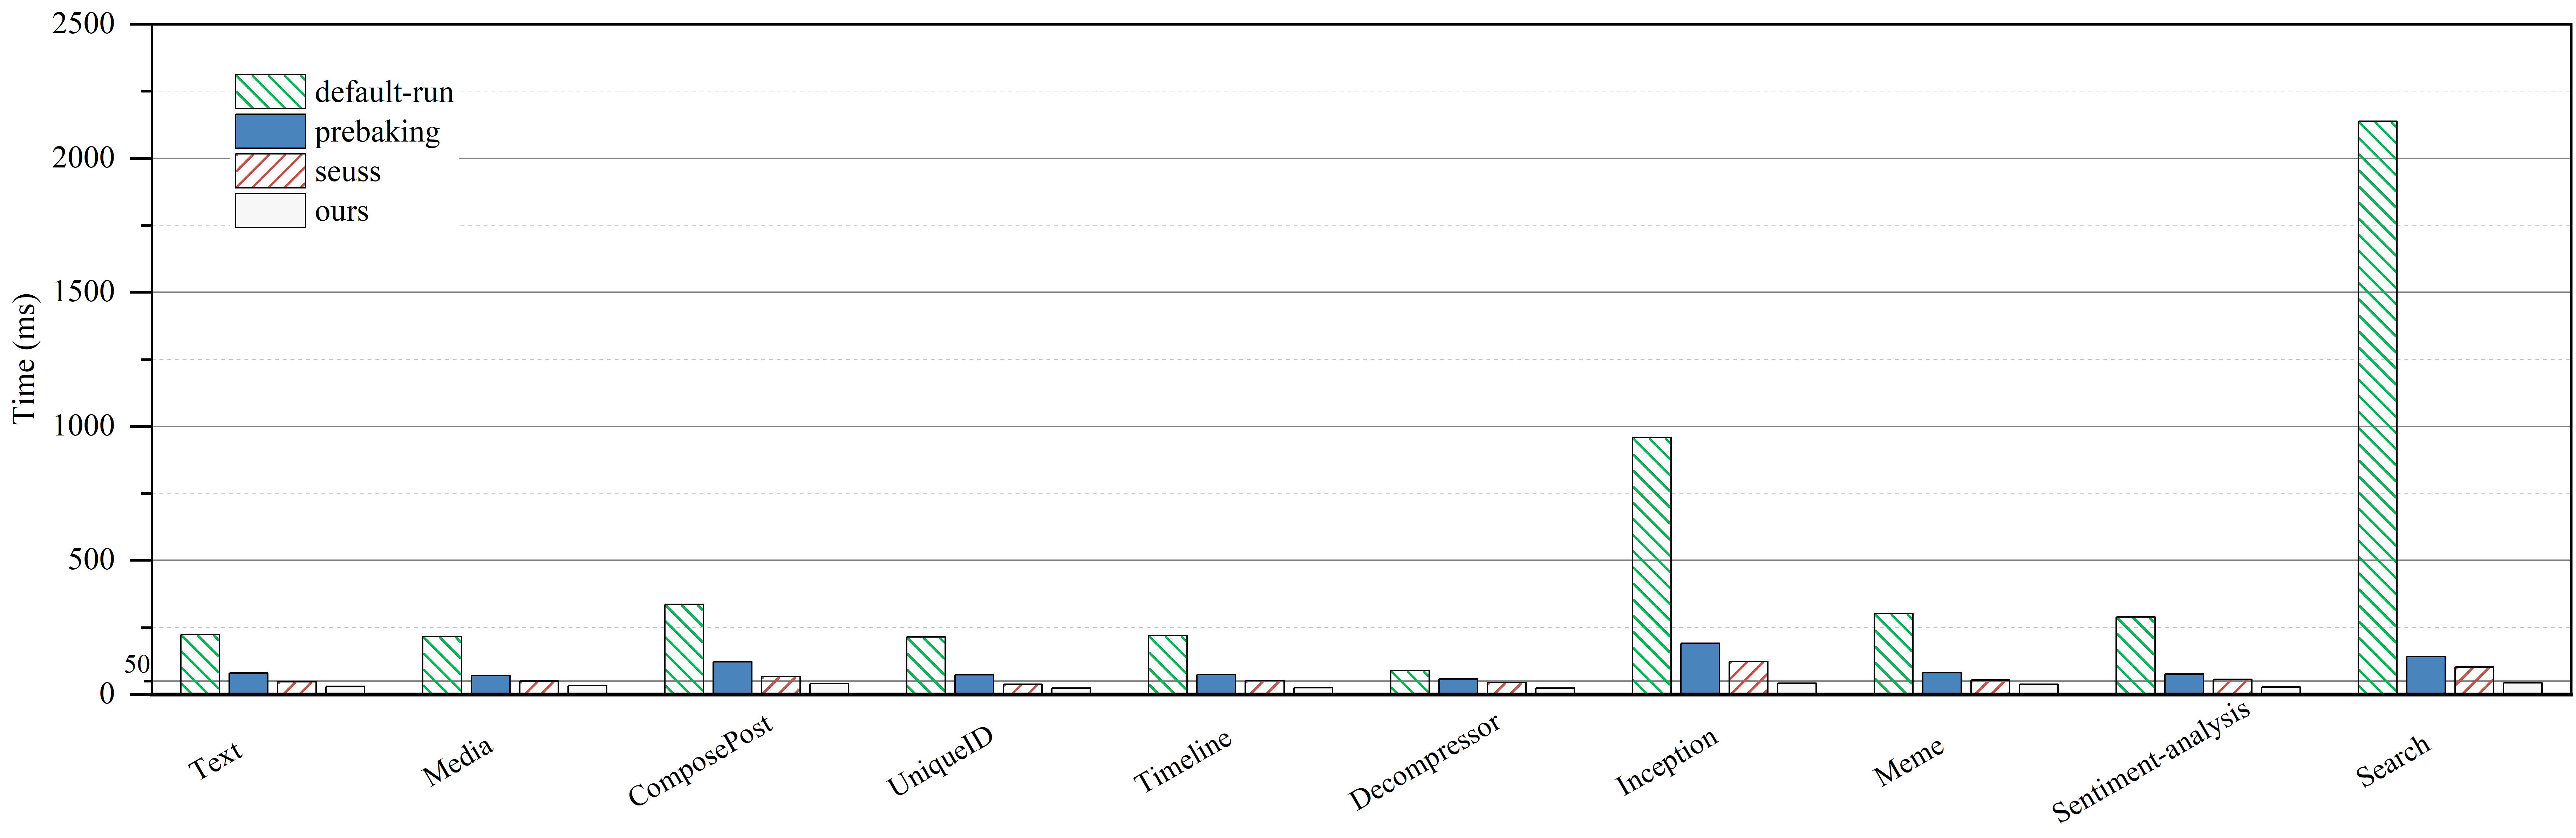
\includegraphics[width=\linewidth]{images/startup-latency.png}
    \caption{Startup latency of serverless functions}
    \label{startup-latency}
\end{figure*}

For \pname, \textit{default-run} and \textit{prebaking}, 
the startup latency on the work node is defined as the time 
interval from the time the runc component receives the request 
to start the serverless function to the time that the 
serverless function is able to handle the coming request; 
for the \textit{seuss}, it is the time interval from when the Rumprun 
system receives the instruction to start the 
serverless function to when the serverless function is started and can accept the request.

The result of the experiment is shown in Figure \ref{startup-latency}. 
The result shows that the serverless function isolation environment pooling strategy and the memory mapping strategy adopted 
in this paper can effectively reduce the function startup latency. 
The startup latency can be reduced by at least 30\% compared to other systems, 
and at least 70\% when compared to the \textit{default-run}.
In addition, the startup latency of all test cases starting by \pname is below 50 milliseconds.

After analyzing the optimized startup phase, 
it can be seen that the isolation environment 
pooling strategy reduces the time spent in the 
isolation environment initialization stage from 
tens of milliseconds to a few milliseconds, 
and the memory mapping strategy also reduces the time spent 
in the memory loading stage to about ten milliseconds.

\subsection{Memory Occupation}

The experiment of the memory occupation uses systems to deploy 
different types of serverless functions, 
and the number of copies of each type of serverless function is 10, 
and the amount of memory used by each function is collected to 
obtain the total amount of memory occupied by all serverless functions of each type.

\begin{figure*}[t]
    \centering
    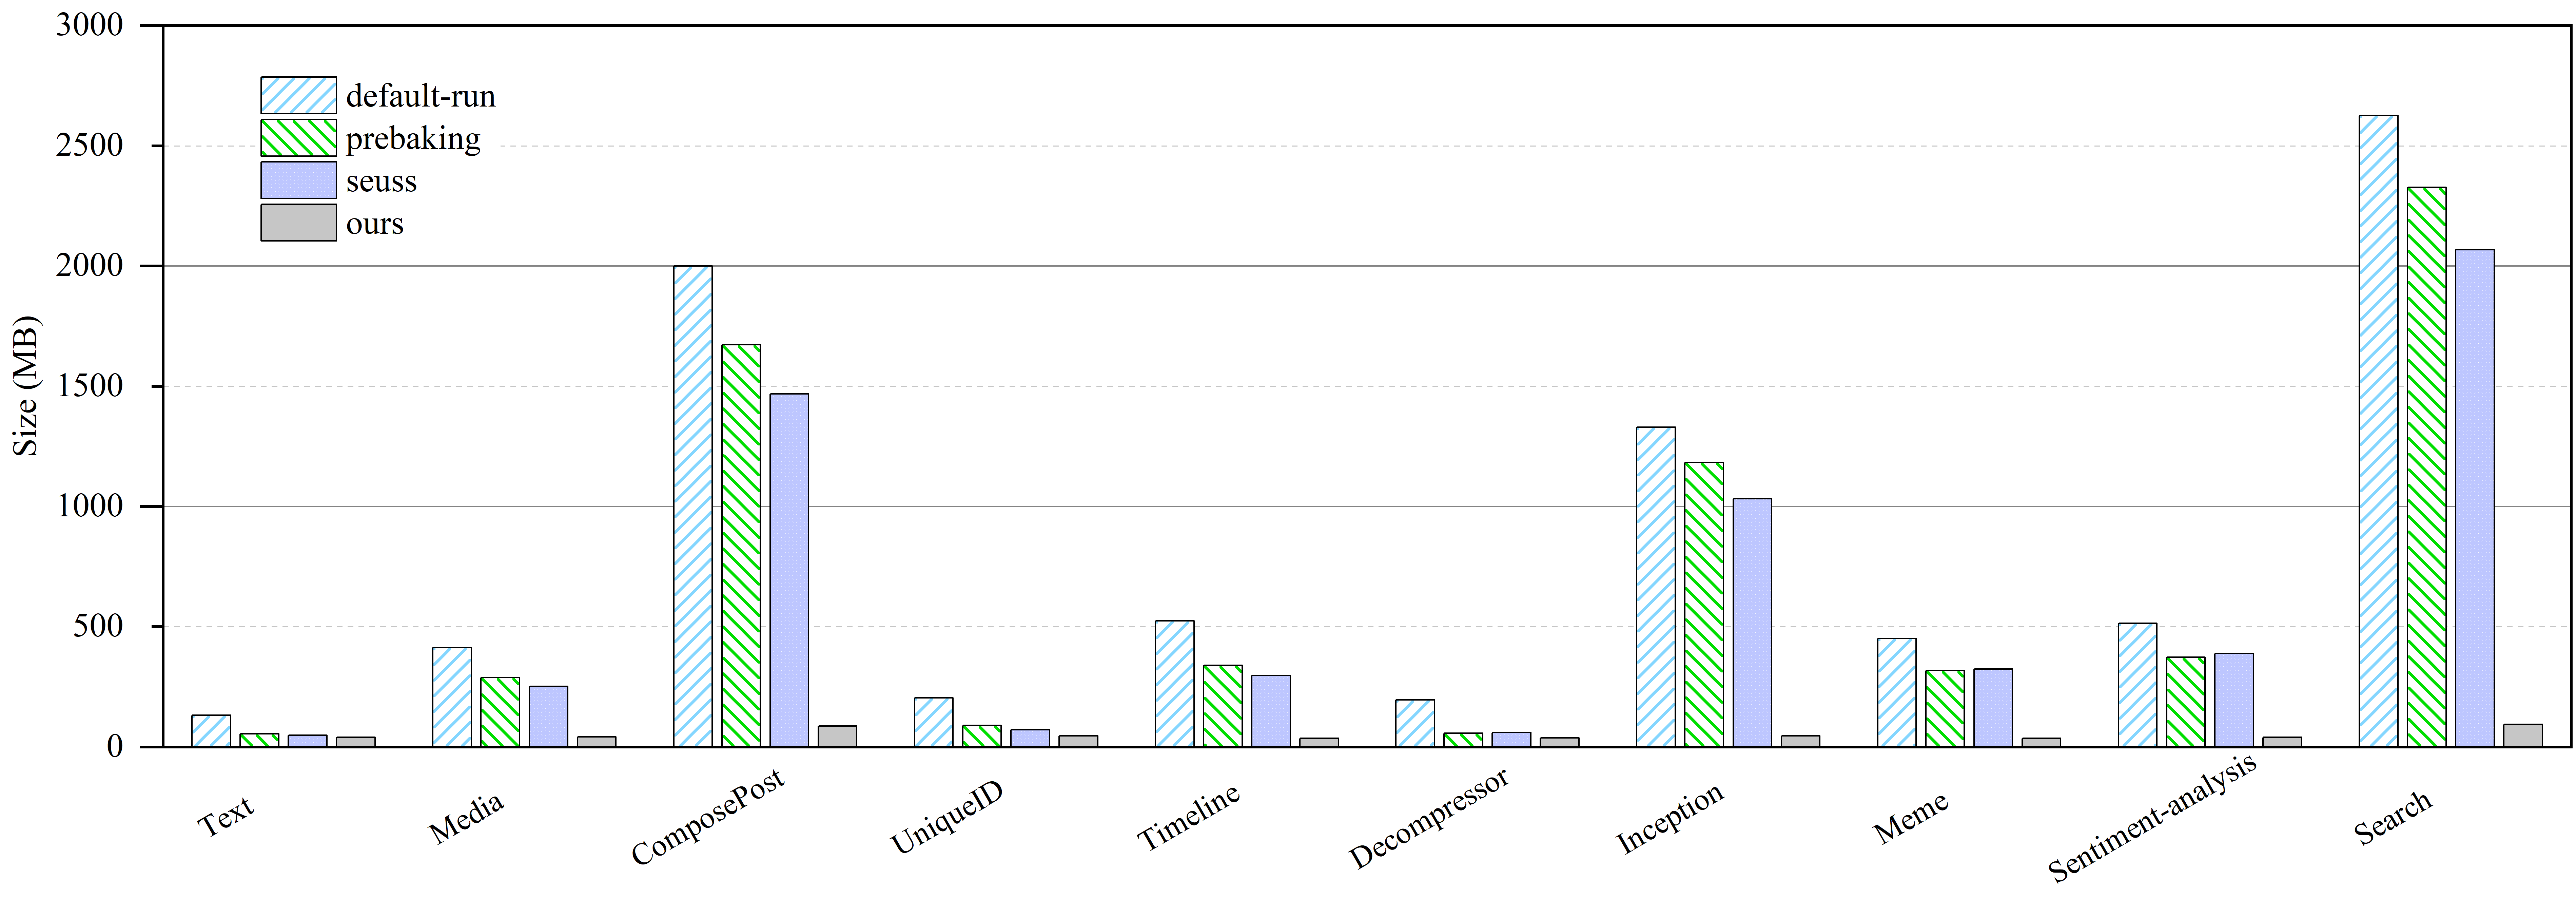
\includegraphics[width=\linewidth]{images/memory.png}
    \caption{Memory footprint of multiple serverless functions}
    \label{memory}
\end{figure*}

The test result(figure \ref{memory}) shows that the use of function memory 
sharing mapping strategy can effectively reduce the resource 
occupation of serverless functions. 
Compared with other systems, 
the total memory occupied by the serverless functions 
deployed by our system is reduced by 20\% to 90\%. 
There is a lot of redundancy in the memory data of the serverless function deployed by other systems, 
but due to the natural isolation between the virtual memory spaces of the process, data cannot be shared, 
resulting in a waste of memory resources.

\subsection{Concurrent Deployment of Serverless Functions}

\begin{figure}[t]
    \centering
    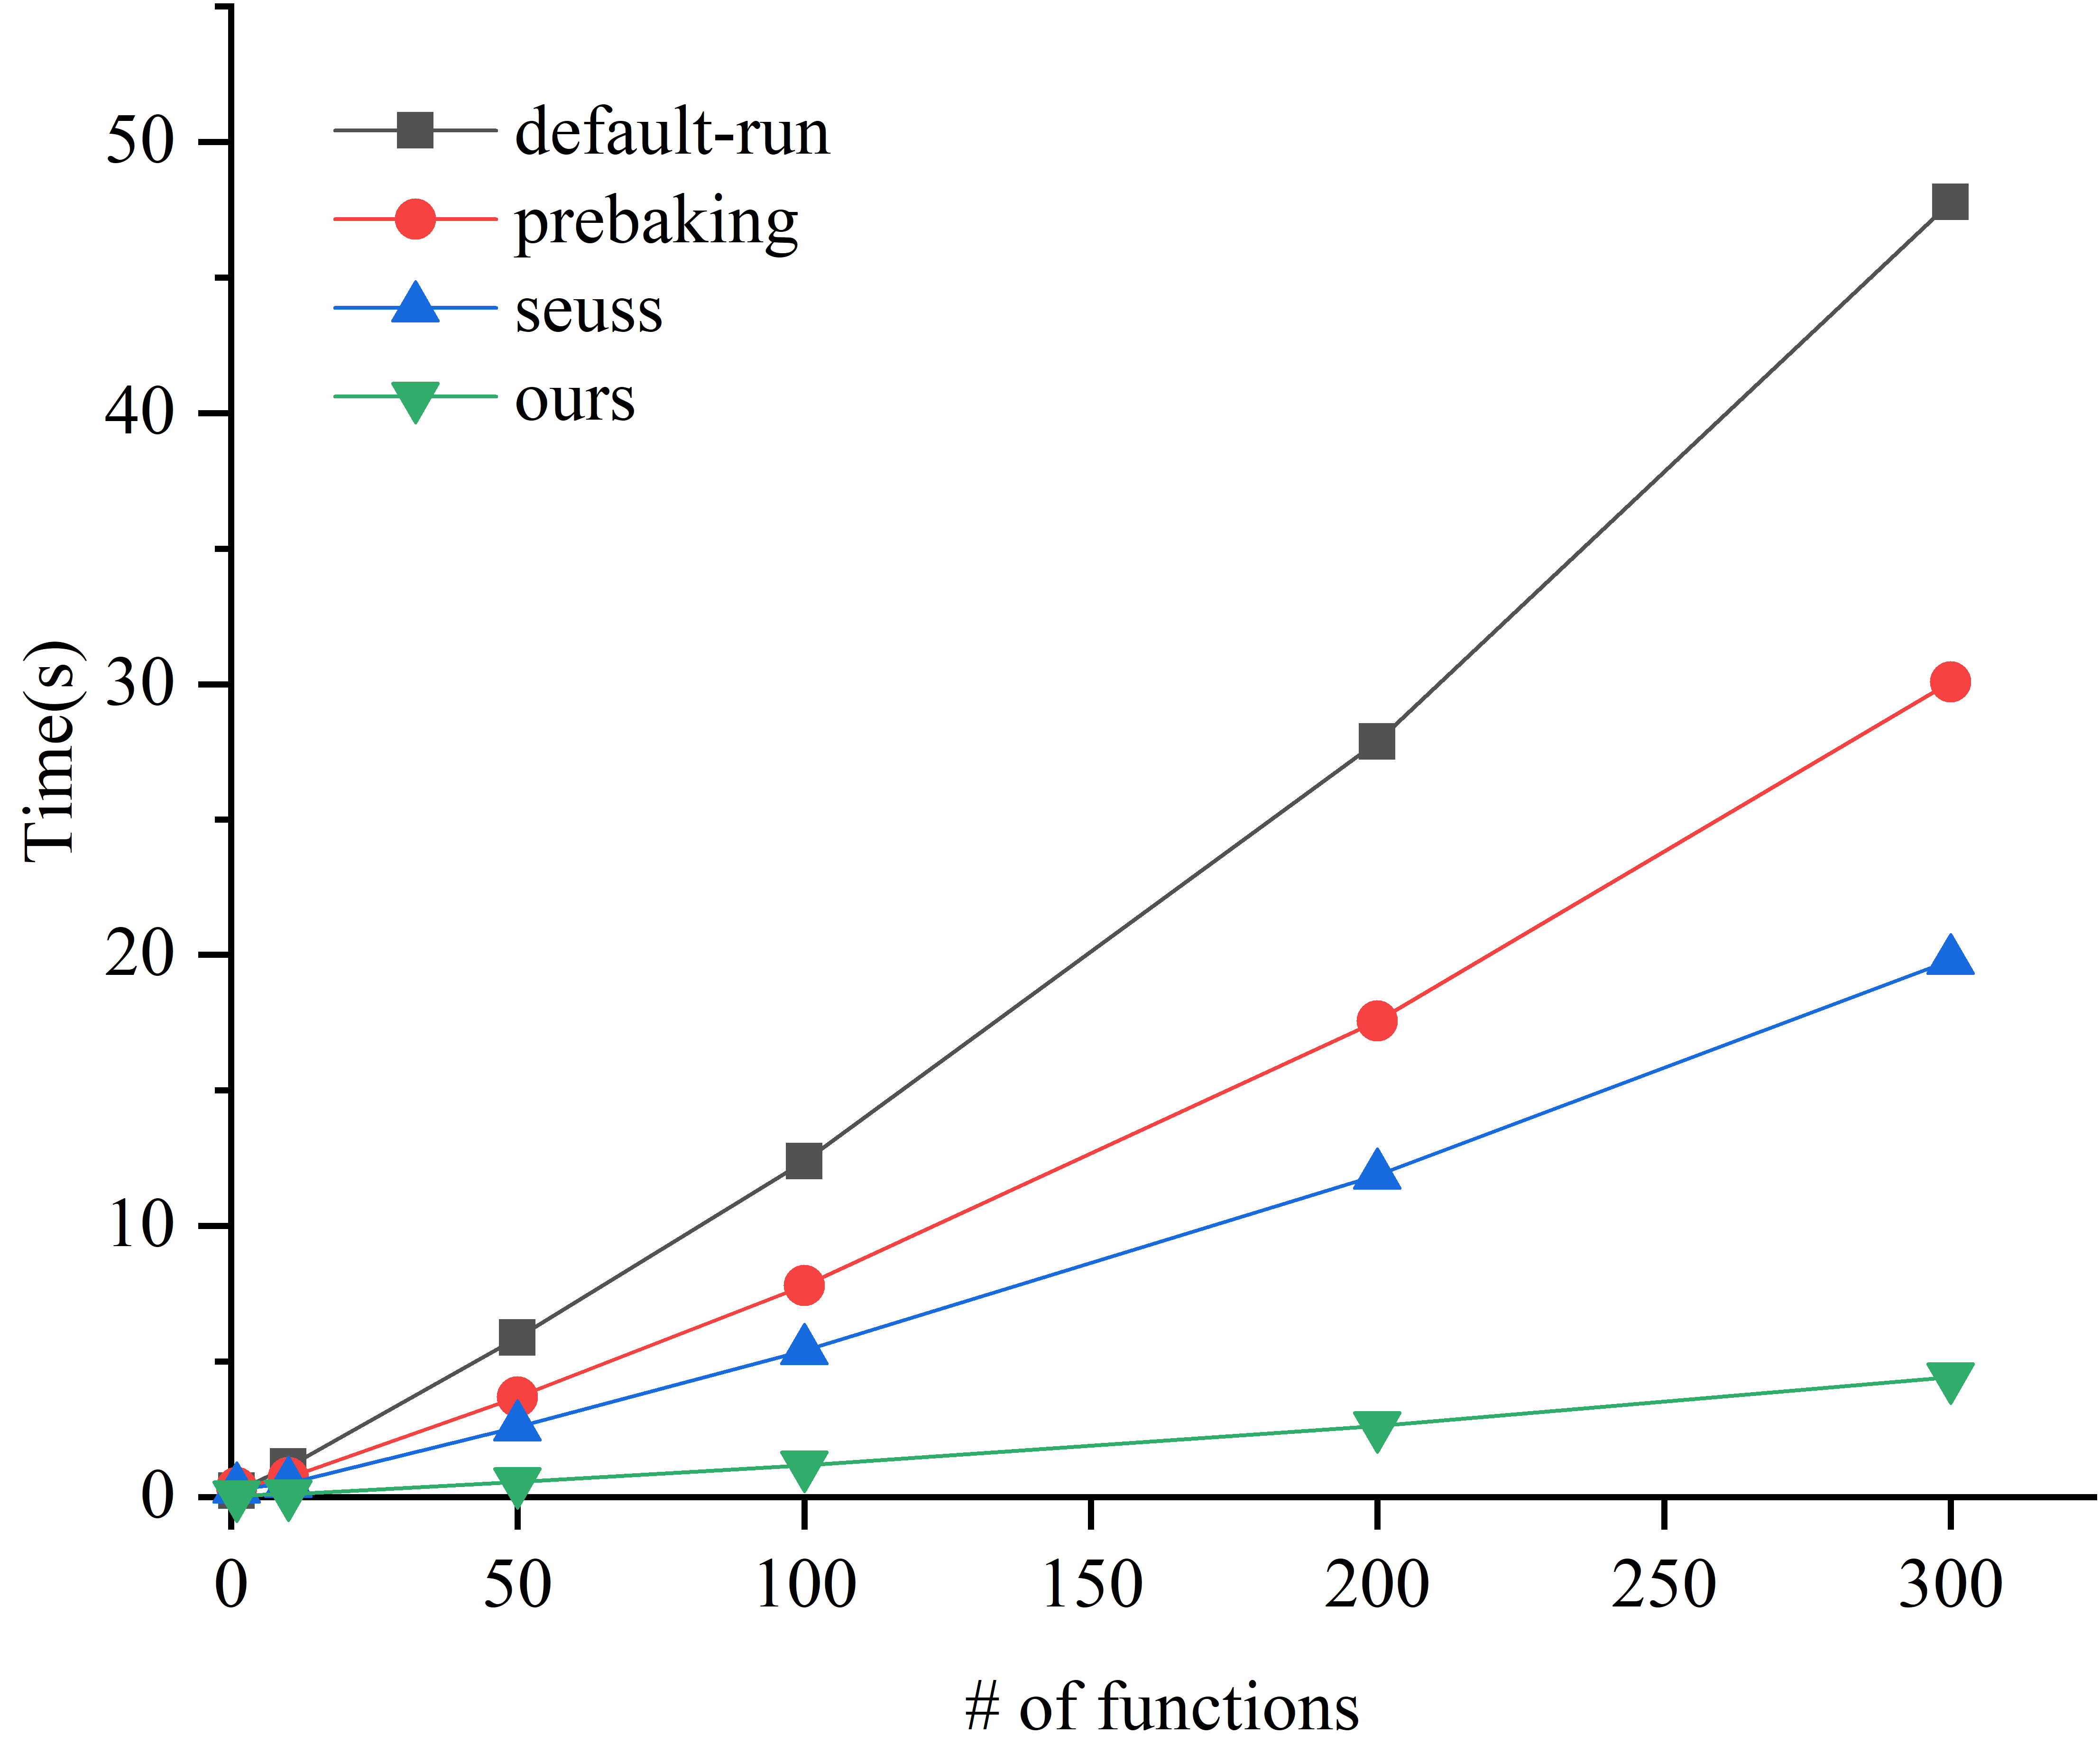
\includegraphics[width=\linewidth]{images/concurrent.png}
    \caption{Latency of current deployment}
    \label{concurrent}
\end{figure}

This experiment uses all systems to deploy serverless functions at a concurrency of 1, 10, 50, 100, 200, and 300. 
The used test cases and their deployment ratio are randomly generated, 
The experimental results are shown in Figure \ref{concurrent}. 
The result shows that compared with the \textit{default-run}, 
our system can save up to 90\% of the deployment time. 
Even compared with other systems, 
the deployment efficiency of our system under high concurrency is also very advantageous. 
This is due to the use of C/S technique to accelerate the startup of serverless functions, at the same time, 
the isolate environment pooling strategy 
and the memory sharing mapping strategy
are adapted to greatly reduce the startup latency. 
In general, 
our system does not have a explosive growth in deployment 
time while the number of functions increases, 
which is conducive to the serverless computing platform to provide services more quickly and efficiently.

\section{related work}

\section{conclusion}
\section*{Acknowledgments}

%%
%% The next two lines define the bibliography style to be used, and
%% the bibliography file.
\bibliographystyle{ACM-Reference-Format}
\bibliography{bibs/refs}

\end{document}
%%
%% End of file `sample-sigconf.tex'.
